\documentclass[journal]{IEEEtran}

% ============================================================
% Packages
% ============================================================

\usepackage{amsmath,amssymb,amsfonts,amsthm}
\usepackage{cite}
\usepackage{algorithmic}
\usepackage{graphicx}
\usepackage{textcomp}
\usepackage{xcolor}
\usepackage{booktabs}
\usepackage{hyperref}
\newtheorem{proposition}{Proposition}
% ============================================================
% Theorem environments
% ============================================================

\newtheorem{theorem}{Theorem}
\newtheorem{lemma}{Lemma}
\newtheorem{definition}{Definition}
% ============================================================
% Document
% ============================================================

\begin{document}
	
	% ============================================================
	% Title
	% ============================================================
	
	\title{FAC-RNN: Fuzzy Adaptive Temporal Scaling with Contractive Recurrent Dynamics for Robust Time-Series Forecasting}
	
	% \author{Author~Name,~Affiliation}
	
	\maketitle
	
	% ============================================================
	% Abstract
	% ============================================================
	
	\begin{abstract}
Recurrent neural networks (RNNs) use a fixed recurrent update mechanism in many forecasting settings, which may limit their ability to adapt to changing temporal dynamics and provides no explicit guarantee on the sensitivity of the recurrent transition. This paper proposes FAC-RNN, a Fuzzy Adaptive Contractive Recurrent Neural Network that introduces context-dependent temporal scaling into the recurrent state update. The proposed model uses an adaptive update rate $\alpha_t$ to control the balance between the previous hidden state and the newly computed recurrent state, while fuzzy rule interpolation provides a smooth bounded mapping from observable temporal context to $\alpha_t$. In addition, an explicit contraction constraint is imposed on the recurrent matrix, $\lVert W_h\rVert_2\leq\kappa<1$, together with a lower bound $\alpha_t\geq\alpha_{\min}>0$. These conditions yield a verifiable one-step Jacobian contraction bound. With $\kappa=0.9$ and $\alpha_{\min}=0.02$, the resulting theoretical bound is $q\leq0.998$. Experiments on controlled nonlinear time-series forecasting show that adaptive temporal scaling provides the main predictive improvement over a fixed update rate, while fuzzy interpolation yields an additional modest gain; however, the latter difference is not statistically significant under the three-seed paired comparison ($p=0.4289$). An external real-world benchmark using monthly Pacific sea-surface-temperature data further shows that FAC-RNN does not uniformly outperform simpler or attention-based baselines, highlighting the distinction between controlled dynamical benefits and broad forecasting generalization. A protocol-matched full-step Jacobian analysis confirms the dynamical distinction: the contractive model exhibits a maximum Jacobian norm of 0.768, with zero observed violations of the unit threshold, whereas the unconstrained counterpart achieves lower MSE but has a maximum Jacobian norm of 1.205 and exceeds the threshold throughout the evaluated trajectory. These results position FAC-RNN as a stability-aware recurrent design with an explicit accuracy--stability trade-off rather than as a uniformly superior forecasting model.
\end{abstract}
	
	% ============================================================
	% Keywords
	% ============================================================
	
	\begin{IEEEkeywords}
		Recurrent Neural Networks,
		Adaptive Temporal Scaling,
		Fuzzy Logic,
		Dynamical Systems,
		Contraction,
		Jacobian Stability,
		Time-Series Forecasting.
	\end{IEEEkeywords}
	
	
	% ============================================================
	% 1. Introduction
	% ============================================================
	
	\section{Introduction}
	\label{sec:introduction}
	
	Recurrent neural networks (RNNs) provide a natural framework for modeling sequential data because their hidden state carries information from previous observations into subsequent time steps. This recurrent structure has made RNNs widely useful for time-series forecasting, where the predictive value of a new observation depends not only on its current magnitude but also on the temporal context accumulated from the past. However, conventional recurrent architectures typically employ a fixed state-transition mechanism, causing every observation to interact with the hidden state through the same update rule. Such a fixed temporal response can be restrictive when the underlying process exhibits changing dynamical characteristics, because different operating regimes may require different degrees of state retention and responsiveness.
	
	One natural way to address this limitation is to introduce an adaptive temporal update mechanism in which the contribution of newly computed information varies with the observed context. Let $\alpha_t$ denote such an adaptive update rate. A small value of $\alpha_t$ places greater emphasis on the previous hidden state and therefore promotes temporal retention, whereas a larger value gives greater weight to the newly computed recurrent state and produces a more responsive update. This interpretation provides a direct dynamical meaning to the recurrent update coefficient and allows the model to adjust its effective temporal scale according to the behavior of the observed sequence.
	
	Although adaptive recurrent mechanisms can improve predictive flexibility, adaptation alone does not provide an explicit guarantee on the sensitivity of the resulting recurrent dynamics. In recurrent systems, the local behavior of the state transition is governed by its Jacobian, and unrestricted recurrent operators may produce transition norms greater than one. Such behavior can increase sensitivity to perturbations and makes it difficult to provide a priori guarantees on the dynamical evolution of the hidden state. This motivates the incorporation of an explicit operator constraint into the recurrent architecture so that predictive adaptation can be combined with a verifiable stability property.
	
	In this work, we propose \emph{FAC-RNN}, a Fuzzy Adaptive Contractive Recurrent Neural Network that combines adaptive temporal scaling with fuzzy context-dependent interpolation and an explicit recurrent contraction constraint. The proposed recurrent transition introduces $\alpha_t$ directly into the state update, thereby allowing the degree of temporal state retention to vary with the observable context. A fuzzy controller maps the current observation and its temporal change to a bounded update rate through smooth interpolation among fuzzy rules. At the same time, the recurrent matrix is constrained by $\lVert W_h\rVert_2\leq\kappa<1$, which enables an analytical bound on the one-step Jacobian.
	
	The controller uses the observable context
	\begin{equation}
		c_t=[y_t,\Delta_t],
		\qquad
		\Delta_t=y_t-y_{t-1},
		\label{eq:intro_context}
	\end{equation}
	rather than the hidden state itself. This design is important because it separates the temporal control signal from the recurrent state being analyzed. As a result, the adaptive coefficient can be treated as fixed with respect to $h_{t-1}$ when deriving the one-step recurrent Jacobian, leading to the tractable form
	\begin{equation}
		J_t=(1-\alpha_t)I+\alpha_tD_tW_h.
		\label{eq:intro_jacobian}
	\end{equation}
	Under the proposed bounds on $\alpha_t$ and $W_h$, this structure yields a uniform contraction condition for the recurrent transition.
	
	The central objective of FAC-RNN is therefore not simply to improve forecasting accuracy, but to establish a recurrent architecture in which predictive adaptation and dynamical control are explicitly separated. The adaptive coefficient determines how quickly the hidden state responds to newly observed information, fuzzy interpolation provides a smooth context-dependent parameterization of this response, and the recurrent contraction constraint limits the sensitivity of the underlying nonlinear transition. This formulation makes it possible to study the predictive and dynamical roles of the proposed components independently.
	
	The experimental evaluation is designed to answer several complementary questions. We first examine whether adaptive temporal scaling improves forecasting performance relative to a fixed update rate. We then isolate the additional contribution of fuzzy interpolation through context ablation and examine whether the learned temporal update rate varies across distinct nonlinear dynamical regimes. We further evaluate data scarcity, external real-world generalization against modern recurrent and attention-based baselines, and the statistical robustness of the observed performance differences. Finally, we compare contractively constrained and unconstrained fuzzy models to quantify the resulting accuracy--stability trade-off and directly evaluate the full-step recurrent Jacobian against the theoretical contraction bound.
	
	The results show that adaptive temporal scaling provides the principal predictive improvement, while fuzzy interpolation yields an additional but smaller gain in the controlled benchmark. In the main forecasting experiment, the proposed fuzzy adaptive model reduces mean test MSE by 12.16\% relative to the fixed update-rate baseline and by 1.66\% relative to the nonfuzzy adaptive model, although the latter paired difference is not statistically significant with three seeds. The learned update rate also exhibits different distributions across the evaluated dynamical regimes, indicating context-dependent temporal modulation. More importantly, with $\kappa=0.9$ and $\alpha_{\min}=0.02$, the proposed architecture admits the theoretical contraction bound
	\begin{equation}
		q\leq0.998<1.
		\label{eq:intro_q}
	\end{equation}
	The protocol-matched full-step Jacobian experiment is consistent with this guarantee, with a maximum observed Jacobian norm of 0.768 for the contractively constrained model and no observed violations of the unit threshold, whereas the unconstrained counterpart achieves lower forecasting error but reaches a maximum Jacobian norm of 1.205 and exceeds the unit threshold throughout the evaluated trajectory.
	
	The contributions of this study can therefore be summarized as follows: first, an adaptive temporal scaling mechanism is embedded directly into the recurrent state transition to regulate the balance between state retention and responsiveness; second, fuzzy rule interpolation is used to obtain a smooth and bounded context-dependent update policy; third, an explicit recurrent contraction constraint is introduced together with a formal Jacobian-based stability guarantee; and fourth, a systematic empirical evaluation distinguishes the predictive contribution of adaptive temporal scaling from the additional fuzzy contribution while explicitly quantifying the trade-off between forecasting accuracy and recurrent dynamical stability.
	
	% ============================================================
	% 2. Related Work
	% ============================================================
	




% ============================================================
% 3. Proposed FAC-RNN
% ============================================================

\section{Proposed FAC-RNN}
\label{sec:method}

The proposed Fuzzy Adaptive Contractive Recurrent Neural Network (FAC-RNN) is designed to jointly address two complementary requirements in recurrent time-series modeling: adaptive temporal responsiveness and controlled recurrent dynamics. The central idea is to replace the conventional fixed recurrent update by a convex state interpolation whose weight is determined dynamically from observable temporal context. A fuzzy controller provides a smooth parameterization of this adaptive update rate, while an explicit constraint on the recurrent transition matrix enables a formal contraction guarantee.

\subsection{Problem Formulation}
\label{subsec:formulation}

Let $\{y_t\}_{t=1}^{T}$ denote a univariate time series and let $x_t\in\mathbb{R}^{d_x}$ denote the input available to the recurrent model at time $t$. Given a lookback window of observations, the objective is to learn a one-step-ahead forecasting function that estimates $y_{t+1}$ from the current input and the recurrent hidden state. In a conventional RNN, the state transition is governed by a fixed nonlinear mapping, which implicitly imposes the same temporal response throughout the sequence. FAC-RNN instead introduces a time-varying update coefficient $\alpha_t$ so that the strength of the recurrent update can depend on the current observable temporal context.

Let $h_t\in\mathbb{R}^{d_h}$ denote the hidden state. FAC-RNN separates the overall mechanism into two coupled but analytically distinguishable components: a recurrent state-transition mechanism that determines the evolution of $h_t$, and a context-dependent controller that determines the scalar temporal update rate $\alpha_t$. The controller is driven exclusively by observable quantities derived from the input sequence. This separation is particularly important for the stability analysis because $\alpha_t$ does not introduce an explicit dependence on $h_{t-1}$ when the one-step recurrent Jacobian is evaluated.

The resulting design provides two complementary capabilities. First, the model can change its effective temporal response according to the local dynamics of the observed sequence. Second, the recurrent operator can be constrained independently of this adaptive controller, allowing a uniform bound on the sensitivity of the recurrent state transition to be established analytically.

\subsection{Recurrent State Update}
\label{subsec:state_update}

The hidden state of FAC-RNN is updated according to

\begin{equation}
	h_t
	=
	(1-\alpha_t)h_{t-1}
	+
	\alpha_t
	\tanh
	\left(
	W_hh_{t-1}+W_xx_t+b_h
	\right),
	\label{eq:fac_update}
\end{equation}

where $W_h\in\mathbb{R}^{d_h\times d_h}$ is the recurrent transition matrix, $W_x\in\mathbb{R}^{d_h\times d_x}$ is the input-to-hidden matrix, $b_h\in\mathbb{R}^{d_h}$ is the recurrent bias, and $\alpha_t$ is the adaptive temporal update rate. The update therefore represents a convex interpolation between the previous hidden state and a newly computed nonlinear recurrent state.

The temporal interpretation of $\alpha_t$ is direct. When $\alpha_t$ is small, the term $(1-\alpha_t)h_{t-1}$ dominates and the hidden state changes slowly, thereby favoring temporal retention. When $\alpha_t$ is large, a greater fraction of the newly computed nonlinear state is incorporated, resulting in a more responsive temporal update. The adaptive coefficient consequently acts as an explicit temporal scaling variable within the recurrent state equation rather than as an auxiliary quantity external to the recurrence.

The forecasting output is obtained from the current hidden state through a linear readout,

\begin{equation}
	\hat{y}_{t+1}
	=
	W_yh_t+b_y,
	\label{eq:fac_output}
\end{equation}

where $W_y$ and $b_y$ denote the output-layer parameters. The complete forecasting function is therefore determined by the recurrent transition together with the context-dependent mechanism that generates $\alpha_t$.

\subsection{Context-Dependent Temporal Scaling}
\label{subsec:temporal_scaling}

The adaptive temporal coefficient is generated from observable temporal context. In the forecasting experiments, the controller input is defined as

\begin{equation}
	c_t
	=
	[y_t,\Delta_t],
	\qquad
	\Delta_t=y_t-y_{t-1},
	\label{eq:context}
\end{equation}

where $y_t$ describes the current signal level and $\Delta_t$ describes its local temporal variation. The use of both quantities provides the controller with information about the current operating point and its short-term evolution without requiring direct access to the hidden state.

The observable context is processed by a compact nonlinear controller to obtain an intermediate scalar score. Specifically, the experimental implementation uses a $2$--$6$--$1$ multilayer mapping,

\begin{equation}
	s_t
	=
	W_{c2}
	\tanh
	\left(
	W_{c1}c_t+b_{c1}
	\right)
	+b_{c2},
	\label{eq:controller_score}
\end{equation}

where $W_{c1}$ and $W_{c2}$ are controller weight matrices and $b_{c1}$ and $b_{c2}$ are the corresponding biases. The scalar score is normalized through

\begin{equation}
	z_t=\tanh(s_t),
	\label{eq:z_definition}
\end{equation}

which produces a bounded latent context variable $z_t\in(-1,1)$ for the subsequent fuzzy interpolation stage.

The separation between the controller and the recurrent state transition is deliberate. The controller determines how strongly the recurrent state should be updated, whereas the recurrent matrix determines the dynamics of the state transition itself. This separation makes it possible to investigate predictive adaptation and dynamical sensitivity as distinct design dimensions.

\subsection{Fuzzy Rule Interpolation}
\label{subsec:fuzzy_interpolation}

The latent variable $z_t$ is mapped to the adaptive update rate using three fuzzy membership functions centered at

\begin{equation}
	\mathcal{C}=\{-1,0,1\}.
	\label{eq:fuzzy_centers}
\end{equation}

For each center $c_i\in\mathcal{C}$, the corresponding Gaussian membership degree is defined as

\begin{equation}
	\mu_i(z_t)
	=
	\exp
	\left(
	-\frac{(z_t-c_i)^2}{2\sigma^2}
	\right),
	\qquad
	i=1,2,3,
	\label{eq:membership}
\end{equation}

where $\sigma>0$ controls the membership width. The width parameter is learned during training using a positive parameterization so that the Gaussian membership functions remain well defined.

The membership degrees are normalized according to

\begin{equation}
	\bar{\mu}_i(z_t)
	=
	\frac{\mu_i(z_t)}
	{\displaystyle\sum_{j=1}^{3}\mu_j(z_t)}.
	\label{eq:normalized_membership}
\end{equation}

Each fuzzy rule is associated with a learnable temporal update value $r_i$. The final adaptive coefficient is obtained through normalized interpolation,

\begin{equation}
	\alpha_t
	=
	\sum_{i=1}^{3}
	\bar{\mu}_i(z_t)r_i.
	\label{eq:fuzzy_interpolation}
\end{equation}

Because the normalized memberships are nonnegative and sum to one, Eq.~\eqref{eq:fuzzy_interpolation} produces a smooth interpolation between neighboring rule values. Unlike a hard rule-selection mechanism, the resulting temporal control signal changes continuously as the observable context changes. This property is particularly suitable for recurrent systems in which abrupt variations in the update coefficient could themselves introduce undesirable changes in the state dynamics.

The fuzzy mechanism is therefore used as a smooth temporal policy parameterization rather than as a separate recurrent memory mechanism. Its role is to provide a context-dependent interpolation of admissible update rates while preserving the bounded structure required by the recurrent state update and the subsequent contraction analysis.

\subsection{Bounded Adaptive Update Rate}
\label{subsec:bounded_alpha}

The adaptive update rate is explicitly constrained to the interval

\begin{equation}
	\alpha_{\min}
	\leq
	\alpha_t
	\leq
	\alpha_{\max}.
	\label{eq:alpha_bounds}
\end{equation}

The experimental configuration uses

\begin{equation}
	\alpha_{\min}=0.02,
	\qquad
	\alpha_{\max}=1.
	\label{eq:alpha_values}
\end{equation}

The lower bound ensures that the newly computed nonlinear state always contributes to the recurrent update, preventing the temporal controller from collapsing to a zero-update state. The upper bound preserves the interpretation of $\alpha_t$ as an interpolation coefficient between the previous and newly computed states.

The fuzzy rule values are parameterized so that the interpolated output remains within this admissible interval. Because the interpolation weights satisfy $\bar{\mu}_i\geq0$ and $\sum_i\bar{\mu}_i=1$, any convex combination of rule outputs within the admissible interval also remains within that interval. Consequently, the temporal controller preserves the bounded update structure required by the recurrent formulation.

\subsection{Contractive Recurrent Parameterization}
\label{subsec:contractive_parameterization}

The adaptive temporal mechanism alone does not impose a bound on the sensitivity of the recurrent transition. FAC-RNN therefore introduces an explicit contraction constraint on the recurrent matrix,

\begin{equation}
	\left\lVert W_h\right\rVert_2
	\leq
	\kappa
	<
	1.
	\label{eq:weight_constraint}
\end{equation}

The experimental value is

\begin{equation}
	\kappa=0.9.
	\label{eq:kappa}
\end{equation}

The constraint limits the operator norm of the recurrent transformation and is enforced during optimization so that the recurrent matrix remains inside the prescribed contractive region. Since the spectral norm is bounded by the Frobenius norm,

\begin{equation}
	\left\lVert W_h\right\rVert_2
	\leq
	\left\lVert W_h\right\rVert_F,
	\label{eq:spectral_fro_bound}
\end{equation}

the implementation uses norm control sufficient to maintain the desired recurrent spectral constraint.

The contraction constraint has a purpose distinct from that of the adaptive controller. The parameter $\alpha_t$ governs the temporal responsiveness of the state update, whereas the constraint on $W_h$ controls the sensitivity of the nonlinear recurrent transformation. This separation allows the architecture to retain adaptive temporal behavior while providing explicit conditions under which the one-step Jacobian can be bounded by a constant smaller than one.

\subsection{Overall FAC-RNN Architecture}
\label{subsec:architecture}

The overall architecture is illustrated in Fig.~\ref{fig:fac_architecture}. At each time step, the observable context $(y_t,\Delta_t)$ is processed by the nonlinear controller to obtain the latent variable $z_t$. The fuzzy membership functions then interpolate the learned rule values to generate the bounded adaptive update rate $\alpha_t$. This coefficient controls the relative contribution of the previous hidden state and the newly computed nonlinear state in Eq.~\eqref{eq:fac_update}, while the recurrent matrix remains subject to the contraction constraint in Eq.~\eqref{eq:weight_constraint}.

\begin{figure}[t]
	\centering
	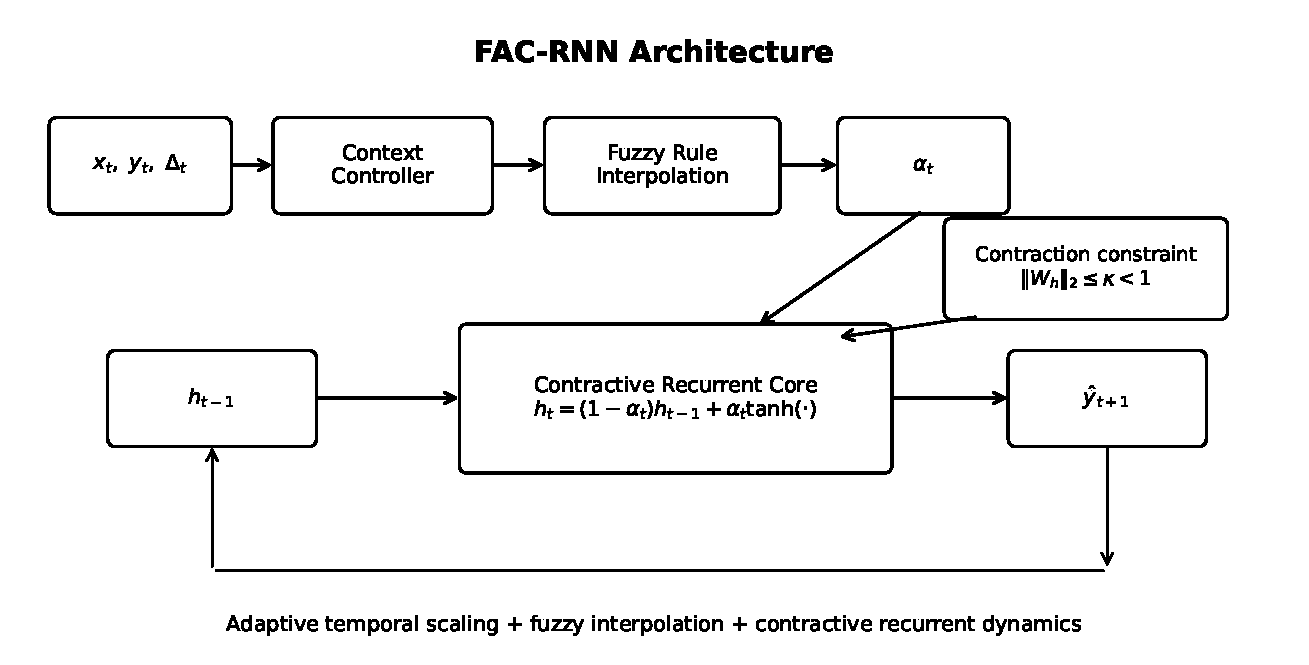
\includegraphics[
	width=\linewidth
	]{paper_figures/Fig1_FAC_RNN_architecture.pdf}
	\caption{Architecture of the proposed FAC-RNN. The observable temporal context $(y_t,\Delta_t)$ is processed by a nonlinear controller to obtain the latent variable $z_t$, which is converted through fuzzy rule interpolation into the bounded adaptive update rate $\alpha_t$. The update rate controls the recurrent state transition, while the recurrent matrix is constrained by $\lVert W_h\rVert_2\leq\kappa<1$.}
	\label{fig:fac_architecture}
\end{figure}

The resulting architecture can be summarized as a sequence of three functional operations: observable temporal context is first transformed into a latent control representation, fuzzy interpolation then determines the adaptive temporal scaling coefficient, and the resulting coefficient modulates a contractively constrained recurrent transition. This decomposition provides the basis for separately analyzing forecasting performance, adaptive temporal behavior, and recurrent dynamical stability in the subsequent experimental sections.


\section{Related Work}

\subsection{Recurrent Neural Networks and Stability}

Recurrent neural networks (RNNs) provide a natural framework for modeling sequential and nonlinear temporal dependencies by maintaining an internal state that evolves over time \cite{bengio1994learning,hochreiter1997long}. However, the repeated application of nonlinear recurrent transformations can lead to vanishing or exploding gradients, making the learning of long-range temporal dependencies difficult \cite{pascanu2013difficulty}. Several approaches have therefore investigated structural or optimization-based mechanisms for controlling recurrent dynamics. Orthogonality and singular-value-based constraints have been proposed to improve gradient propagation and regulate the recurrent transition matrix \cite{vorontsov2017orthogonality,zhang2018svd}. These approaches explicitly regulate recurrent matrix properties to improve gradient propagation and control recurrent sensitivity. More recently, random orthogonal constructions and structured recurrent architectures have further explored ways of improving the numerical behavior of recurrent systems \cite{ceni2025random}. These studies emphasize the importance of controlling recurrent dynamics, but they generally treat stability and predictive adaptation as separate design objectives.

Dynamical approaches have also been proposed in which stability is incorporated more explicitly into the recurrent formulation. Continuous-time-inspired recurrent models such as coRNN impose structural restrictions on the recurrent dynamics to obtain desirable long-term behavior \cite{rusch2021corNN}, while the Lipschitz Echo State Model provides stability-oriented recurrent dynamics through controlled state transitions \cite{erichson2021lipschitz}. Lyapunov-based recurrent constructions have similarly demonstrated that stability conditions can be integrated directly into the learning architecture rather than being considered only as a post-training diagnostic \cite{vogt2022lyapunov}. These studies motivate the use of explicit dynamical constraints in recurrent forecasting models, but they do not directly address the combination of adaptive temporal scaling, fuzzy context-dependent interpolation, and an explicit contraction guarantee considered in FAC-RNN.

\subsection{Adaptive Temporal Scales in Recurrent Models}

An important limitation of conventional RNNs is that a single fixed recurrent update rate may be poorly suited to temporal processes that contain heterogeneous or changing dynamics. Adaptive recurrent formulations have consequently introduced learnable time constants or update rates so that different components can respond at different temporal scales. Quax et al. showed that learnable time constants can improve recurrent modeling and enable the recovery of multiple characteristic temporal scales from data \cite{quax2020adaptivetimescales}. Similarly, Tanaka et al. demonstrated that recurrent systems with diverse leak rates can represent multiscale dynamics more effectively than models relying on a single fixed time scale \cite{tanaka2022reservoir}. These findings provide strong motivation for making the recurrent update rate adaptive rather than fixed.

Related work has also explored continuous-time and liquid-style recurrent architectures in which the effective temporal dynamics vary according to the current context \cite{hasani2021ltc}. The common principle across these approaches is that temporal responsiveness should be adapted to the evolving signal rather than imposed uniformly across all observations. FAC-RNN follows this general direction but differs in how the adaptation is constructed: the update coefficient $\alpha_t$ is produced by an observable-context controller and then regularized through a bounded fuzzy interpolation mechanism. This formulation is specifically designed to provide both adaptive temporal behavior and an analytically tractable contraction condition.

\subsection{Adaptive Recurrent Learning and Stability}

Adaptive recurrent learning has also been studied from a control-theoretic perspective. Agand et al. developed adaptive recurrent structures whose update rules are derived using discrete-time Lyapunov arguments, showing that adaptation can be incorporated while maintaining stability properties of the resulting system \cite{agand2017adaptive}. This line of work is particularly relevant to FAC-RNN because it demonstrates that recurrent adaptation and dynamical stability need not be treated as independent objectives. However, the adaptation mechanism in such approaches is fundamentally different from the context-dependent fuzzy interpolation employed here.

More recently, recurrent equilibrium formulations have provided explicit conditions under which recurrent transformations can remain well behaved and converge to stable representations \cite{revay2024recurrent}. Such models strengthen the connection between recurrent learning and formal dynamical analysis. Nevertheless, equilibrium-based formulations primarily focus on the properties of the recurrent operator or its fixed point, whereas FAC-RNN uses an explicit adaptive interpolation coefficient within the recurrent state update and derives a direct contraction bound for each input-conditioned hidden-state transition.

\subsection{Fuzzy and Neuro-Fuzzy Recurrent Models}

Fuzzy systems provide a complementary mechanism for representing nonlinear relationships through interpretable local rules and smooth interpolation between operating regions. Neuro-fuzzy recurrent models have been developed to combine the representation capabilities of neural networks with fuzzy rule-based adaptation. Global stability properties have been investigated for fuzzy recurrent systems, demonstrating that fuzzy nonlinearities can be incorporated while preserving desirable dynamical characteristics \cite{zhu2011global}. Other studies have considered synchronization and nonlinear control problems using fuzzy or recurrent fuzzy structures, further illustrating the usefulness of fuzzy adaptation for nonlinear dynamical systems \cite{mohammadzadeh2015synchronization}.

Recent work has continued to develop adaptive recurrent neuro-fuzzy architectures. For example, the PTFA-RNN framework integrates fuzzy processing with recurrent learning to improve adaptive sequence modeling \cite{cheng2025ptfar}. Related developments in monotone and structured fuzzy systems have emphasized constraints on nonlinear mappings that can improve interpretability and analytical properties \cite{teh2018monotone,kerk2025monotone}. These studies support the use of fuzzy mechanisms for context-dependent nonlinear adaptation, but the role of fuzzy rules in FAC-RNN is deliberately narrower. The fuzzy component does not replace the recurrent dynamics; instead, it smoothly maps a low-dimensional observable context to the bounded update coefficient $\alpha_t$. This separation makes it possible to analyze the recurrent contraction independently of the complexity of the fuzzy controller.

\subsection{Contractive and Lipschitz-Constrained Recurrent Dynamics}

A growing body of research has investigated Lipschitz constraints and contractive mappings as a means of obtaining stable neural dynamics. Lipschitz-constrained neural architectures explicitly control the sensitivity of network transformations to their inputs, providing a useful mathematical framework for analyzing robustness and stability \cite{erichson2021lipschitz}. In recurrent settings, constraining the recurrent operator is particularly important because the same transformation is repeatedly applied over time; even a modest expansion factor can therefore become significant over long horizons. Spectral, orthogonal, and norm-based constraints have consequently been explored as mechanisms for controlling recurrent sensitivity \cite{vorontsov2017orthogonality,zhang2018svd}.

FAC-RNN adopts a direct contractive formulation by constraining the recurrent matrix according to $\|W_h\|_2\leq\kappa<1$ while simultaneously enforcing a strictly positive lower bound on the adaptive update coefficient, $\alpha_t\geq\alpha_{\min}>0$. Because the controller depends only on the observable context rather than the hidden state, the resulting one-step Jacobian admits a particularly simple analytical form. This allows a direct norm bound on the hidden-state transition and consequently a multi-step contraction bound. In contrast to approaches that use stability only as an empirical regularizer or post-training property, the contraction requirement in FAC-RNN is incorporated into the model definition itself.

\subsection{Positioning of FAC-RNN}

The literature therefore reveals three closely related but largely separate research directions. The first develops adaptive temporal mechanisms that allow recurrent systems to operate at multiple or context-dependent time scales \cite{quax2020adaptivetimescales,tanaka2022reservoir,hasani2021ltc}. The second investigates fuzzy and neuro-fuzzy recurrent mechanisms for nonlinear and interpretable adaptation \cite{teh2018monotone,kerk2025monotone}. The third focuses on explicit dynamical control through Lyapunov, Lipschitz, spectral, or contractive constraints \cite{agand2017adaptive,erichson2021lipschitz,revay2024recurrent,vogt2022lyapunov}. However, the combination of adaptive temporal scaling, fuzzy context-dependent interpolation, and an explicit recurrent contraction guarantee remains comparatively less explored in a unified lightweight forecasting architecture.

FAC-RNN is positioned at this intersection. Its contribution is not the introduction of adaptive recurrence, fuzzy inference, or contraction theory in isolation, but their coordinated integration into a single forecasting architecture. The adaptive coefficient $\alpha_t$ provides context-dependent temporal scaling, fuzzy interpolation supplies a smooth nonlinear mapping from observable signal context to the update rate, and the recurrent spectral constraint provides an explicit contraction guarantee. This design enables the study of a concrete research question that is difficult to isolate in conventional recurrent models: to what extent can adaptive temporal control improve forecasting accuracy while an explicit contraction constraint simultaneously limits recurrent sensitivity? The experiments in this work therefore evaluate not only predictive performance, but also ablations, regime adaptation, data scarcity, and the empirical relationship between forecasting accuracy and recurrent stability.

% ============================================================
% 4. Dynamical Stability Analysis
% ============================================================

\section{Dynamical Stability Analysis}
\label{sec:stability}

\subsection{One-Step Jacobian}
\label{subsec:jacobian}

Consider the recurrent transition defined in~\eqref{eq:fac_update}. Let $u_t=W_hh_{t-1}+W_xx_t+b_h$ denote the pre-activation vector and define $D_t=\operatorname{diag}(1-\tanh^2(u_t))$. Since the adaptive coefficient $\alpha_t$ is generated from the observable context $c_t=[y_t,\Delta_t]$ and does not explicitly depend on $h_{t-1}$, it is treated as fixed when differentiating the recurrent transition with respect to the previous hidden state. Therefore, the one-step Jacobian of the hidden-state transition is given by

\begin{equation}
	J_t
	=
	\frac{\partial h_t}{\partial h_{t-1}}
	=
	(1-\alpha_t)I
	+
	\alpha_tD_tW_h.
	\label{eq:jacobian}
\end{equation}

The matrix $D_t$ contains the local derivatives of the hyperbolic tangent activation. Since $0<1-\tanh^2(u)\leq1$ for every finite component of $u$, its spectral norm satisfies

\begin{equation}
	\left\lVert D_t\right\rVert_2
	\leq1.
	\label{eq:D_norm}
\end{equation}

Equation~\eqref{eq:jacobian} separates the recurrent sensitivity into an identity contribution weighted by $(1-\alpha_t)$ and a nonlinear recurrent contribution weighted by $\alpha_t$. This decomposition is central to the contraction analysis because both terms are explicitly controlled by the bounded update rate and the recurrent matrix norm.

% ------------------------------------------------------------
% 4.2 Jacobian Norm Bound
% ------------------------------------------------------------

\subsection{Jacobian Norm Bound}
\label{subsec:jacobian_bound}

Applying the triangle inequality and the submultiplicative property of the spectral norm to~\eqref{eq:jacobian} gives

\begin{align}
	\left\lVert J_t\right\rVert_2
	&\leq
	\left\lVert(1-\alpha_t)I\right\rVert_2
	+
	\left\lVert\alpha_tD_tW_h\right\rVert_2
	\nonumber\\
	&=
	(1-\alpha_t)
	+
	\alpha_t
	\left\lVert D_tW_h\right\rVert_2
	\nonumber\\
	&\leq
	(1-\alpha_t)
	+
	\alpha_t
	\left\lVert D_t\right\rVert_2
	\left\lVert W_h\right\rVert_2.
	\label{eq:jacobian_bound_step1}
\end{align}

Using~\eqref{eq:D_norm} and the recurrent contraction constraint in~\eqref{eq:weight_constraint}, we obtain

\begin{equation}
	\left\lVert J_t\right\rVert_2
	\leq
	(1-\alpha_t)+\alpha_t\kappa
	=
	1-\alpha_t(1-\kappa).
	\label{eq:jacobian_bound_step2}
\end{equation}

Because $\alpha_t\geq\alpha_{\min}>0$, the right-hand side can be uniformly bounded by

\begin{equation}
	\left\lVert J_t\right\rVert_2
	\leq
	1-\alpha_{\min}(1-\kappa)
	=:q.
	\label{eq:uniform_q}
\end{equation}

Since $\kappa<1$ and $\alpha_{\min}>0$, it follows that

\begin{equation}
	0\leq q<1.
	\label{eq:q_less_one}
\end{equation}

Thus, every admissible one-step recurrent transition is a contraction in the Euclidean norm.

% ------------------------------------------------------------
% 4.3 Contraction Theorem
% ------------------------------------------------------------

\subsection{Contraction Theorem}
\label{subsec:contraction_theorem}

\begin{theorem}
	Suppose that the recurrent matrix satisfies $\left\lVert W_h\right\rVert_2\leq\kappa<1$ and that the adaptive temporal update rate satisfies $\alpha_t\geq\alpha_{\min}>0$ for all time steps. Then the FAC-RNN one-step state-transition map is contractive with contraction factor
	
	\begin{equation}
		q
		=
		1-\alpha_{\min}(1-\kappa)
		<
		1,
		\label{eq:theorem_q}
	\end{equation}
	
	and consequently satisfies $\left\lVert J_t\right\rVert_2\leq q$ for every admissible state and input.
	
\end{theorem}

\begin{proof}
	For any fixed input $x_t$ and observable controller context, consider two hidden states $h_{t-1}^{(1)}$ and $h_{t-1}^{(2)}$. Since $\alpha_t$ is determined by the observable context, the corresponding one-step transition has the Jacobian~\eqref{eq:jacobian}. By~\eqref{eq:jacobian_bound_step2},
	
	\begin{equation}
		\left\lVert J_t\right\rVert_2
		\leq
		1-\alpha_t(1-\kappa).
	\end{equation}
	
	Because $\alpha_t\geq\alpha_{\min}$ and $1-\kappa>0$,
	
	\begin{equation}
		1-\alpha_t(1-\kappa)
		\leq
		1-\alpha_{\min}(1-\kappa)
		=
		q.
	\end{equation}
	
	Hence $\left\lVert J_t\right\rVert_2\leq q<1$. By the mean-value inequality, the corresponding state-transition map is Lipschitz continuous with Lipschitz constant at most $q$, and therefore is contractive. \hfill$\square$
\end{proof}
	% ------------------------------------------------------------
	% 4.4 Numerical Contraction Bound
	% ------------------------------------------------------------
	
	\subsection{Numerical Contraction Bound}
	\label{subsec:numerical_bound}
	
	For the experimental configuration used in this study, the recurrent contraction parameter is set to $\kappa=0.9$ and the minimum adaptive update rate is set to $\alpha_{\min}=0.02$. Substituting these values into~\eqref{eq:theorem_q} gives
	
	\begin{equation}
		q
		=
		1-\alpha_{\min}(1-\kappa)
		=
		1-0.02(1-0.9)
		=
		0.998.
		\label{eq:numerical_q}
	\end{equation}
	
	Therefore,
	
	\begin{equation}
		\boxed{
			\left\lVert J_t\right\rVert_2
			\leq
			0.998
			<
			1
		}
		\label{eq:final_contraction_bound}
	\end{equation}
	
	for every admissible recurrent transition satisfying the imposed parameter constraints. This bound is conservative because it is obtained from the worst-case inequalities $\left\lVert D_t\right\rVert_2\leq1$ and $\left\lVert W_h\right\rVert_2\leq\kappa$, whereas the realized Jacobian norm can be substantially smaller along a particular trajectory.
	
	% ------------------------------------------------------------
	% 4.5 Multi-Step Consequence
	% ------------------------------------------------------------
	
	\subsection{Multi-Step Consequence}
	\label{subsec:multistep}
	
	Let $J_{t:t+L}$ denote the Jacobian of the hidden state after $L$ recurrent transitions with respect to the hidden state at time $t$. By the chain rule,
	
	\begin{equation}
		J_{t:t+L}
		=
		J_{t+L}J_{t+L-1}\cdots J_{t+1}.
		\label{eq:jacobian_product}
	\end{equation}
	
	Using the submultiplicative property of the spectral norm and the uniform bound in~\eqref{eq:final_contraction_bound}, we obtain
	
	\begin{equation}
		\left\lVert J_{t:t+L}\right\rVert_2
		\leq
		\prod_{k=t+1}^{t+L}
		\left\lVert J_k\right\rVert_2
		\leq
		q^L.
		\label{eq:multistep_bound}
	\end{equation}
	
	Since $0\leq q<1$, the multi-step sensitivity therefore decays geometrically with the number of recurrent transitions. In particular,
	
	\begin{equation}
		\lim_{L\rightarrow\infty}
		\left\lVert J_{t:t+L}\right\rVert_2
		=
		0.
		\label{eq:asymptotic_jacobian}
	\end{equation}
	
	This result establishes a bound on the sensitivity of the hidden-state dynamics to perturbations in the previous hidden state over arbitrary recurrent horizons. Importantly, this is a statement about the recurrent state-transition dynamics and should not be interpreted as a direct guarantee on task-level forecasting error.
	
	% ------------------------------------------------------------
	% 4.6 Interpretation of the Stability Guarantee
	% ------------------------------------------------------------
	
	\subsection{Interpretation of the Stability Guarantee}
	\label{subsec:stability_interpretation}
	
	The stability mechanism in FAC-RNN is distinct from the predictive adaptation mechanism. The adaptive coefficient $\alpha_t$ determines the temporal response of the hidden state to new information, while the constraint on $W_h$ limits the sensitivity of the recurrent nonlinear transformation. The lower bound on $\alpha_t$ and the upper bound on the recurrent spectral norm jointly produce a uniform contraction factor that is independent of the particular hidden-state trajectory.
	
	The theoretical guarantee also clarifies the role of the contraction constraint in the experiments. The constraint is not introduced to minimize the forecasting loss directly; instead, it restricts the recurrent dynamics to a region in which a formal contraction bound can be established. Consequently, an unconstrained model may achieve lower predictive error while failing to satisfy the same dynamical guarantee. The experimental analysis in Section~\ref{sec:results} evaluates this accuracy--stability trade-off through direct full-step Jacobian measurements.
	
	
\begin{proposition}[Sensitivity bound of the fuzzy temporal policy]
	Consider the fuzzy temporal controller used in FAC-RNN with rule
	centers $c_i\in\{-1,0,1\}$, rule values
	$r_i\in[\alpha_{\min},\alpha_{\max}]$, and Gaussian membership width
	$\sigma>0$. Let
	\[
	\alpha(z)=\sum_{i=1}^{3} w_i(z)r_i,
	\]
	where the normalized membership weights are
	\[
	w_i(z)=
	\frac{
		\exp\left(-\frac{(z-c_i)^2}{2\sigma^2}\right)
	}{
		\sum_{j=1}^{3}
		\exp\left(-\frac{(z-c_j)^2}{2\sigma^2}\right)
	}.
	\]
	Then the fuzzy policy satisfies
	\[
	\left|\frac{d\alpha}{dz}\right|
	\leq
	\frac{\alpha_{\max}-\alpha_{\min}}{2\sigma^2}.
	\]
	Furthermore, for the controller
	\[
	z=\tanh\left(
	W_2\tanh(W_1c+b_1)+b_2
	\right),
	\]
	its observable-context sensitivity satisfies
	\[
	\left\|
	\frac{\partial\alpha}{\partial c}
	\right\|_2
	\leq
	\frac{\alpha_{\max}-\alpha_{\min}}
	{2\sigma^2}
	\|W_2\|_2\|W_1\|_2.
	\]
\end{proposition}

\begin{proof}
	The normalized Gaussian memberships can be rewritten as a softmax
	distribution whose logits are
	\[
	\ell_i(z)=\frac{zc_i}{\sigma^2}
	-\frac{c_i^2}{2\sigma^2}.
	\]
	Therefore,
	\[
	\frac{dw_i}{dz}
	=
	\frac{w_i}{\sigma^2}
	(c_i-\bar c),
	\qquad
	\bar c=\sum_{j=1}^{3}w_jc_j.
	\]
	Hence,
	\[
	\frac{d\alpha}{dz}
	=
	\frac{1}{\sigma^2}
	\sum_{i=1}^{3}
	w_i(r_i-\bar r)(c_i-\bar c),
	\]
	which is the weighted covariance between $r$ and $c$ divided by
	$\sigma^2$. Since the ranges of $r_i$ and $c_i$ are respectively
	$\alpha_{\max}-\alpha_{\min}$ and $2$, the covariance is bounded by
	their product divided by four. Thus,
	\[
	\left|\frac{d\alpha}{dz}\right|
	\leq
	\frac{\alpha_{\max}-\alpha_{\min}}
	{2\sigma^2}.
	\]
	Moreover, since the derivative of $\tanh$ is bounded by one,
	\[
	\left\|
	\frac{\partial z}{\partial c}
	\right\|_2
	\leq
	\|W_2\|_2\|W_1\|_2.
	\]
	The chain rule therefore gives
	\[
	\left\|
	\frac{\partial\alpha}{\partial c}
	\right\|_2
	\leq
	\frac{\alpha_{\max}-\alpha_{\min}}
	{2\sigma^2}
	\|W_2\|_2\|W_1\|_2.
	\]
\end{proof}


% ============================================================
% 5. Experimental Design
% ============================================================

\section{Experimental Design}
\label{sec:experiments}

\subsection{Nonlinear Time-Series Generator}
\label{subsec:data_generator}

To evaluate the forecasting behavior of FAC-RNN under changing temporal dynamics, we construct a deterministic nonlinear time series containing three distinct dynamical regimes. The series contains $24{,}000$ observations and is generated once using a fixed random seed of 2026 to ensure reproducibility across all experiments. Each regime has a length of 800 time steps and is generated from a different nonlinear autoregressive mechanism with additive Gaussian noise of standard deviation 0.03. The three regimes represent a slowly varying nonlinear oscillator, a faster nonlinear oscillator, and a nonlinear autoregressive process, respectively.

The first regime is generated according to

\begin{equation}
	y_t
	=
	0.94y_{t-1}
	-0.08y_{t-2}
	+0.10\sin(0.055t+0.7y_{t-1})
	+\varepsilon_t,
	\label{eq:regime_a}
\end{equation}

whereas the second regime is generated according to

\begin{equation}
	y_t
	=
	0.72y_{t-1}
	+0.12y_{t-2}
	+0.22\sin(0.16t+1.2y_{t-1})
	+\varepsilon_t.
	\label{eq:regime_b}
\end{equation}

The third regime introduces an explicit nonlinear autoregressive term and is defined as

\begin{equation}
	y_t
	=
	0.62y_{t-1}
	+0.08y_{t-2}
	-0.10y_{t-1}^{3}
	+0.14\sin(0.095t+0.8y_{t-1})
	+\varepsilon_t.
	\label{eq:regime_c}
\end{equation}

Here, $\varepsilon_t\sim\mathcal{N}(0,0.03^2)$ denotes the additive noise term. The use of multiple nonlinear regimes provides a controlled setting in which the temporal response required by the recurrent model can vary over time while maintaining a common forecasting task.

\subsection{Data Splitting and Forecasting Protocol}
\label{subsec:protocol}

All experiments use a chronological split to avoid information leakage from future observations into the training process. The full series is divided into 60\% training, 20\% validation, and 20\% test segments, corresponding to 14,400, 4,800, and 4,800 observations, respectively. A lookback window of 64 observations is used to construct the recurrent input sequences, and the prediction target is the observation immediately following each input window.

For the main forecasting experiments, 9,000 training windows, 2,500 validation windows, and 2,500 test windows are used. The windows are extracted chronologically from the corresponding data partitions, and the same forecasting protocol is applied to all compared models. Input normalization is fitted using the training observations only and the resulting transformation is then applied to the validation and test observations. This procedure ensures that information from the validation and test partitions is not used when estimating the preprocessing parameters.

The main forecasting comparison is repeated using three independent random seeds, $\{42,123,456\}$, while the underlying generated time series remains fixed. The use of multiple seeds allows the reported performance to reflect variation caused by model initialization and stochastic optimization rather than a single training realization.

\subsection{Real-World Benchmark Protocol}
\label{subsec:realworld_protocol}

As an external validation experiment, we evaluate all models on the El Nino monthly sea-surface-temperature dataset available through the \texttt{statsmodels} data collection. The dataset contains 61 years of monthly Pacific Ocean sea-surface-temperature observations from 1950 to 2010, corresponding to 732 monthly observations in total, and the underlying source is the NOAA National Weather Service ERSST.V3B Nino 1+2 series~\cite{seabold2010statsmodels}. The data are unrolled in chronological monthly order and divided into 60\% training, 20\% validation, and 20\% test observations, yielding 439, 146, and 147 observations, respectively. A lookback window of 24 months is used for one-step-ahead forecasting, and normalization is fitted using the training observations only.

The external benchmark uses five independent random seeds, $\{42,123,456,789,2026\}$. To accommodate the smaller dataset while keeping the comparison controlled, all models use a hidden dimension of 32, Adam optimization with learning rate $10^{-3}$ and weight decay $10^{-4}$, gradient clipping at 1.0, a maximum of 50 epochs, and early stopping with a patience of eight epochs. The Transformer baseline uses two encoder layers with four attention heads and a feed-forward dimension of 64. This benchmark is intended as an external generalization test rather than as a replacement for the controlled nonlinear-regime experiments.

\subsection{Models and Baselines}
\label{subsec:baselines}

The main comparison considers three recurrent configurations that differ in how the temporal update rate is determined. The first baseline uses a fixed update rate and therefore does not adapt its temporal response to the observed context. The second baseline uses a learned nonfuzzy adaptive update rate driven by the observable temporal context. The third model is the proposed FAC-RNN, in which the same adaptive temporal mechanism is parameterized through fuzzy rule interpolation and combined with the contractive recurrent constraint.

To isolate the contribution of the fuzzy mechanism, an additional context ablation is performed using four configurations: fixed $\alpha$, learned value-only control, learned value-plus-$\Delta$ control, and fuzzy value-plus-$\Delta$ control. This design separates the effect of adaptive temporal scaling from the additional effect of fuzzy interpolation.

A separate stability ablation compares the contractively constrained fuzzy model with an otherwise comparable unconstrained fuzzy model. This comparison is used to characterize the predictive cost or benefit associated with explicitly constraining the recurrent dynamics and to distinguish forecasting accuracy from the dynamical stability guarantee.

For the real-world benchmark, the baseline set is expanded to include LSTM and GRU recurrent models~\cite{hochreiter1997long,cho2014gru} and a Transformer encoder~\cite{vaswani2017attention}. These models are evaluated using the same chronological split, lookback horizon, preprocessing rule, optimizer family, and seed protocol as the FAC-RNN benchmark, with architecture-specific hidden dimensions matched to the external benchmark setting.

\subsection{Training Configuration}
\label{subsec:training}

All recurrent models use a hidden dimension of 48 and are trained with mini-batches of 128 windows. The optimization uses Adam with an initial learning rate of $10^{-3}$ and weight decay of $10^{-4}$. Training is performed for a maximum of 15 epochs with early stopping based on validation MSE using a patience of four epochs. Gradient norms are clipped to 1.0 to avoid excessively large parameter updates during optimization.

For the adaptive temporal controller, the update rate is bounded by $\alpha_{\min}=0.02$ and $\alpha_{\max}=1.0$. The recurrent contraction parameter is set to $\kappa=0.90$. The fuzzy controller uses three Gaussian membership functions centered at $-1$, $0$, and $1$, with a learned positive membership width. Unless otherwise stated, all compared models use the same training protocol, forecasting windows, optimization settings, and random seeds.

\subsection{Evaluation Metrics}
\label{subsec:metrics}

Forecasting performance is evaluated using mean squared error (MSE) as the primary metric and mean absolute error (MAE) as a complementary measure. For a sequence of $N$ test predictions, MSE and MAE are defined as

\begin{equation}
	\mathrm{MSE}
	=
	\frac{1}{N}
	\sum_{t=1}^{N}
	\left(
	\hat{y}_t-y_t
	\right)^2,
	\label{eq:mse}
\end{equation}

and

\begin{equation}
	\mathrm{MAE}
	=
	\frac{1}{N}
	\sum_{t=1}^{N}
	\left|
	\hat{y}_t-y_t
	\right|.
	\label{eq:mae}
\end{equation}

The dynamical behavior of the recurrent models is evaluated using the spectral norm of the recurrent matrix, the full-step Jacobian spectral norm, and the number or fraction of evaluated time steps for which the Jacobian norm exceeds one. The latter measures provide direct empirical evidence for whether the observed recurrent transition remains within the contractive region predicted by the theoretical analysis.

For the stability experiments, the analytical full-step Jacobian is additionally cross-checked against an automatic-differentiation Jacobian. The maximum absolute discrepancy between the two calculations is reported as a numerical verification of the Jacobian implementation rather than as an additional performance metric.

\subsection{Experimental Questions}
\label{subsec:research_questions}

The experimental design is organized around five questions. First, does adaptive temporal scaling improve forecasting accuracy relative to a fixed update rate? Second, what additional predictive contribution is obtained by fuzzy interpolation beyond a nonfuzzy adaptive controller? Third, does the learned update rate exhibit different behavior across the distinct dynamical regimes? Fourth, what accuracy--stability trade-off results from imposing the explicit contraction constraint? Fifth, do direct full-step Jacobian measurements empirically support the theoretical contraction guarantee derived in Section~\ref{sec:stability}?
	
	
	% ============================================================
	% 6. Results
	% ============================================================
	
	\section{Results}
	\label{sec:results}
	
	\subsection{Main Forecasting Performance}
	\label{subsec:main_results}
	
	The main forecasting results are summarized in Table~\ref{tab:main_forecasting} and visualized in Fig.~\ref{fig:forecasting_comparison}. The fixed update-rate baseline obtains a mean test MSE of 0.008253 $\pm$ 0.000237, whereas the nonfuzzy adaptive model reduces the error to 0.007372 $\pm$ 0.000198. The proposed fuzzy adaptive model achieves the lowest mean MSE among the contractively constrained models, at 0.007250 $\pm$ 0.000018. Relative to the fixed baseline, the fuzzy adaptive model reduces the mean test error by 12.16\%, while the reduction relative to the nonfuzzy adaptive model is 1.66\%. However, the paired comparison across the three seeds yields $p=0.0207$ for fuzzy versus fixed and $p=0.4289$ for fuzzy versus nonfuzzy; the latter difference should therefore be regarded as a modest descriptive improvement rather than statistically significant evidence of superiority.
	
	\begin{table}[t]
		\centering
		\caption{Main forecasting performance over the three evaluated seeds. Values are mean test MSE $\pm$ standard deviation.}
\label{tab:main_forecasting}
\begin{tabular}{lcc}
\toprule
Model & Test MSE $\pm$ SD & Improvement vs. Fixed \\
\midrule
Fixed $\alpha$ & 0.008253 $\pm$ 0.000237 & -- \\
Nonfuzzy adaptive $\alpha$ & 0.007372 $\pm$ 0.000198 & 10.68\% \\
Fuzzy adaptive $\alpha$ & \textbf{0.007250 $\pm$ 0.000018} & \textbf{12.16\%} \\
\bottomrule
\end{tabular}
	\end{table}
	
	These results indicate that the principal predictive benefit comes from allowing the temporal update rate to adapt rather than remaining fixed. The additional improvement obtained by fuzzy interpolation is smaller than the gain produced by adaptive temporal scaling itself, but it remains positive in the main comparison. This distinction is important because it separates the contribution of temporal adaptation from the contribution of fuzzy parameterization.
	
	\begin{figure}[t]
		\centering
		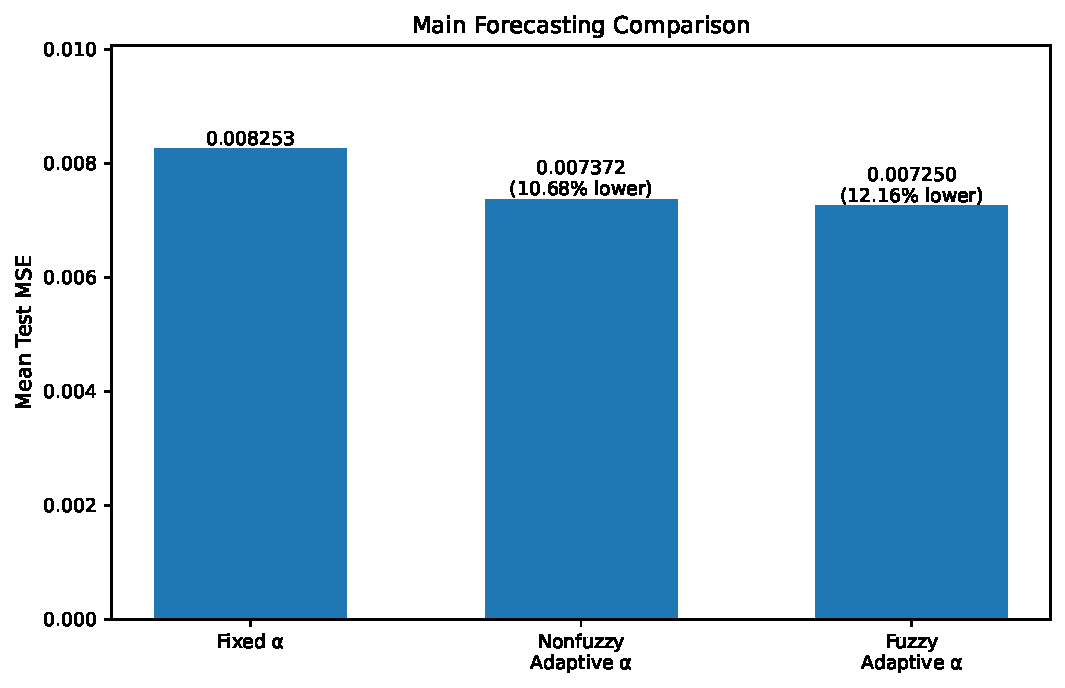
\includegraphics[
		width=0.90\linewidth
		]{paper_figures/Fig3_forecasting_comparison.pdf}
		\caption{Main forecasting comparison. Adaptive temporal scaling reduces the test MSE relative to the fixed update-rate baseline, while fuzzy interpolation provides an additional improvement over the nonfuzzy adaptive controller.}
		\label{fig:forecasting_comparison}
	\end{figure}
	
	% ------------------------------------------------------------
	% 6.2 Context Ablation
	% ------------------------------------------------------------
	
	\subsection{Context Ablation}
	\label{subsec:context_ablation_results}
	
	The contribution of adaptive context processing and fuzzy interpolation is further examined through the context ablation in Table~\ref{tab:context_ablation}. The fixed-$\alpha$ configuration obtains a mean test MSE of 0.008883. Learning the update rate from the observable value reduces the MSE to 0.007694, demonstrating that adaptive temporal scaling provides the dominant improvement. Adding the temporal difference $\Delta_t$ to the nonfuzzy controller changes the mean MSE only slightly, from 0.007694 to 0.007679. Replacing the nonfuzzy mapping with fuzzy interpolation further reduces the MSE to 0.007518, corresponding to a 2.10\% improvement over the matched nonfuzzy value-plus-$\Delta$ configuration.
	
	\begin{table}[t]
		\centering
		\caption{Context ablation results.}
		\label{tab:context_ablation}
		\begin{tabular}{lc}
			\toprule
			Model & Mean Test MSE \\
			\midrule
			Fixed $\alpha$ & 0.008883 \\
			Learned value-only & 0.007694 \\
			Learned value+$\Delta$ & 0.007679 \\
			Fuzzy value+$\Delta$ & \textbf{0.007518} \\
			\bottomrule
		\end{tabular}
	\end{table}
	
	The ablation therefore supports a hierarchical interpretation of the proposed architecture. The largest performance change is associated with replacing the fixed temporal update by an adaptive mechanism, whereas the addition of fuzzy interpolation contributes a smaller but measurable improvement. The limited difference between the value-only and value-plus-$\Delta$ nonfuzzy configurations also indicates that the temporal-difference input alone is not responsible for the main predictive gain.
	
	% ------------------------------------------------------------
	% 6.3 Adaptive alpha across regimes
	% ------------------------------------------------------------
	
	\subsection{Adaptive Temporal Scaling Across Dynamical Regimes}
	\label{subsec:alpha_regimes_results}
	
	The learned temporal update rate exhibits different distributions across the three dynamical regimes, as shown in Fig.~\ref{fig:adaptive_alpha_regimes}. The observed mean values are 0.3909 for Regime~0, 0.4234 for Regime~1, and 0.3893 for Regime~2. The higher mean update rate in Regime~1 is consistent with a greater temporal responsiveness in that regime, while the lower means in Regimes~0 and~2 indicate relatively slower average updates.
	
	\begin{figure}[t]
		\centering
		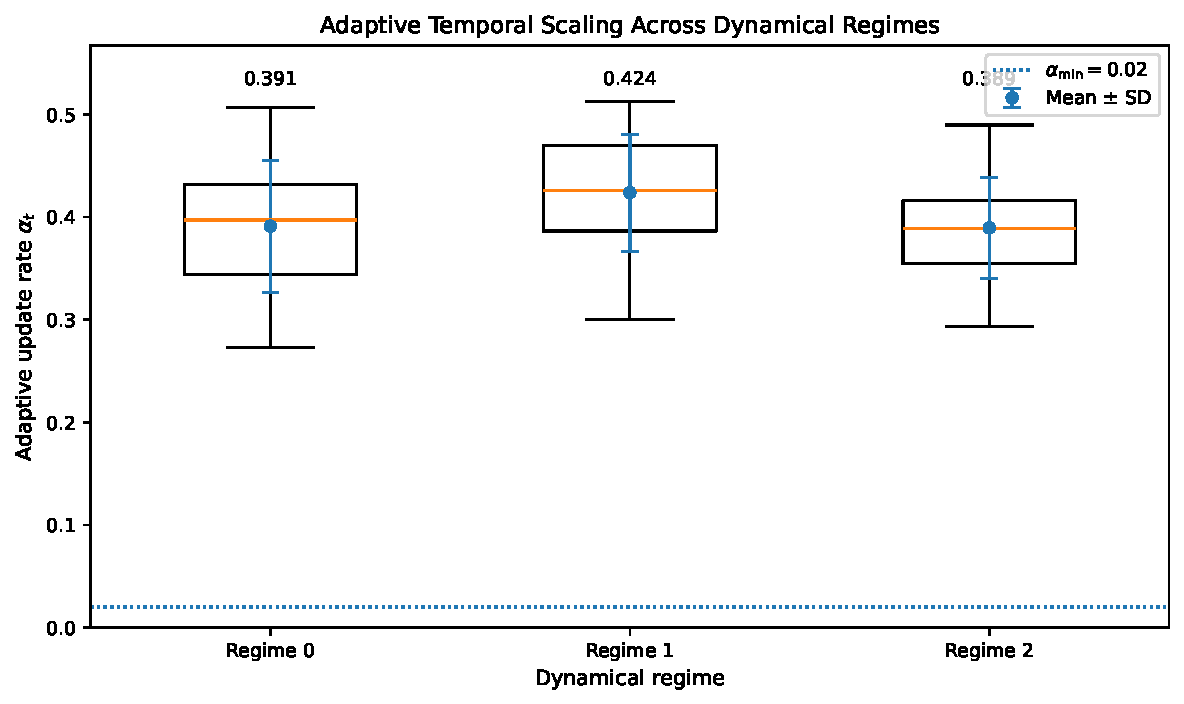
\includegraphics[
		width=0.95\linewidth
		]{paper_figures/Fig2_adaptive_alpha_regimes.pdf}
		\caption{Distribution of the adaptive temporal update rate $\alpha_t$ across the three dynamical regimes. The boxplots summarize the within-regime distributions, while markers and error bars show the mean and standard deviation. The observed regime means are approximately 0.391, 0.424, and 0.389, respectively.}
		\label{fig:adaptive_alpha_regimes}
	\end{figure}
	
	The regime-dependent behavior demonstrates that the learned update rate is not constant across the input dynamics. Instead, the controller produces a context-dependent temporal response. However, the present results do not establish that fuzzy interpolation detects regime transitions faster than the nonfuzzy controller, and therefore the contribution is interpreted as adaptive temporal modulation rather than explicitly faster regime detection.
	
	% ------------------------------------------------------------
	% 6.4 Fuzzy Policy Analysis
	% ------------------------------------------------------------
	
	\subsection{Fuzzy Policy Analysis}
	\label{subsec:fuzzy_policy_results}
	
	The learned fuzzy policy is visualized in Fig.~\ref{fig:fuzzy_policy}. The surface maps the observable context $(y_t,\Delta_t)$ to the adaptive update rate $\alpha_t$ and exhibits a smooth variation across the evaluated input domain. This behavior is a direct consequence of normalized fuzzy rule interpolation, which combines neighboring rule values continuously rather than selecting a single discrete rule.
	
	\begin{figure}[t]
		\centering
		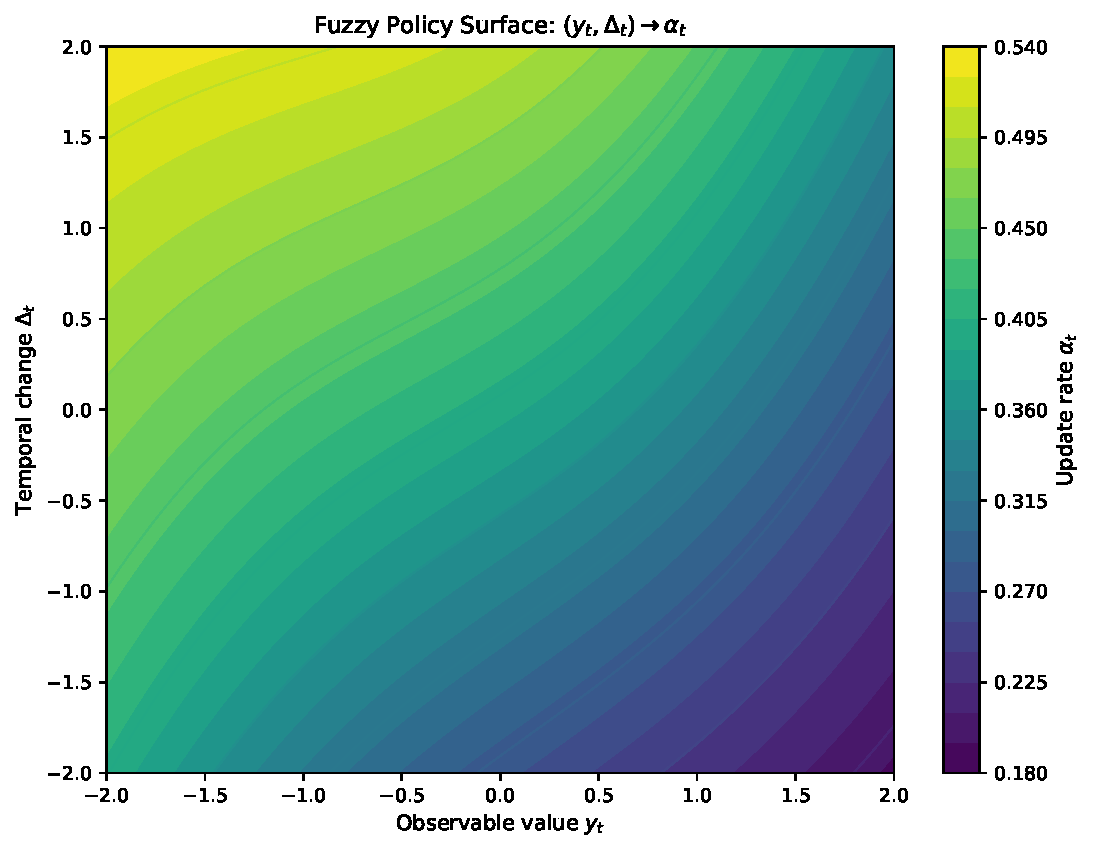
\includegraphics[
		width=0.95\linewidth
		]{paper_figures/Fig4_fuzzy_policy.pdf}
		\caption{Learned fuzzy policy surface mapping the observable context $(y_t,\Delta_t)$ to the adaptive temporal update rate $\alpha_t$. The smooth surface illustrates the bounded context-dependent temporal scaling produced by fuzzy rule interpolation.}
		\label{fig:fuzzy_policy}
	\end{figure}
	
	The learned policy remains within the prescribed admissible interval for the update rate. The resulting smooth mapping provides a continuous temporal control mechanism and illustrates how different observable contexts can induce different degrees of recurrent state updating. The figure should therefore be interpreted as evidence of a smooth learned policy rather than as a proof of any particular semantic interpretation of the fuzzy rules.
	
	% ------------------------------------------------------------
	% 6.5 Regime Shift Performance
	% ------------------------------------------------------------
	
	\subsection{Performance Under Regime Shifts}
	\label{subsec:regime_shift_results}
	
	The regime-shift experiment provides an additional evaluation of adaptive temporal modulation. The fixed-$\alpha$ model obtains a test MSE of 0.010442, while the nonfuzzy adaptive model reduces the error to 0.008768. The fuzzy adaptive model achieves 0.008631, corresponding to a further 1.57\% reduction relative to the nonfuzzy adaptive configuration.
	
	\begin{table}[t]
		\centering
		\caption{Forecasting performance under changing dynamical regimes.}
		\label{tab:regime_shift}
		\begin{tabular}{lc}
			\toprule
			Model & Test MSE \\
			\midrule
			Fixed $\alpha$ & 0.010442 \\
			Nonfuzzy adaptive $\alpha$ & 0.008768 \\
			Fuzzy adaptive $\alpha$ & \textbf{0.008631} \\
			\bottomrule
		\end{tabular}
	\end{table}
	
	The results are consistent with the intended role of the adaptive temporal coefficient. Both adaptive models outperform the fixed-rate baseline, and the fuzzy model provides a modest additional improvement. The result supports the ability of the proposed architecture to modulate its temporal response across different dynamical conditions without requiring a fixed update rate for all regimes.
	
	% ------------------------------------------------------------
	% 6.6 Data Scarcity
	% ------------------------------------------------------------
	
	\subsection{Data-Scarcity Analysis}
	\label{subsec:data_scarcity_results}
	
	The data-scarcity experiment evaluates the effect of reducing the number of training windows while keeping the evaluation protocol unchanged. As shown in Table~\ref{tab:data_scarcity}, the fixed update-rate baseline deteriorates sharply as the number of training windows decreases, with its test MSE increasing from 0.008795 at 9,000 windows to 0.173803 at 1,000 windows. The adaptive nonfuzzy model is substantially more robust, obtaining MSE values of 0.007714, 0.008678, 0.009828, and 0.018869 for 9,000, 5,000, 3,000, and 1,000 windows, respectively.
	
	\begin{table}[t]
		\centering
		\caption{Test MSE under reduced training-set sizes.}
		\label{tab:data_scarcity}
		\begin{tabular}{rccc}
			\toprule
			Training windows & Fixed $\alpha$ & Nonfuzzy $\alpha$ & Fuzzy $\alpha$ \\
			\midrule
			1,000 & 0.173803 & \textbf{0.018869} & 0.043039 \\
			3,000 & 0.019363 & \textbf{0.009828} & 0.010428 \\
			5,000 & 0.011250 & \textbf{0.008678} & 0.008790 \\
			9,000 & 0.008795 & 0.007714 & \textbf{0.007599} \\
			\bottomrule
		\end{tabular}
	\end{table}
	
	The fuzzy model does not consistently outperform the nonfuzzy adaptive model at the smallest training sizes. At 1,000 windows, for example, the fuzzy configuration obtains 0.043039 compared with 0.018869 for the nonfuzzy adaptive model. At the full 9,000-window setting, however, the fuzzy model obtains the best result, with an MSE of 0.007599. These observations indicate that adaptive temporal scaling is the more robust source of improvement under limited data, whereas fuzzy interpolation is not uniformly superior under extreme data scarcity. The preceding sensitivity analysis provides a structural characterization of this finite-sample behavior. For the fuzzy temporal policy, the context sensitivity is bounded by
	\[
	L_F
	\leq
	\frac{\alpha_{\max}-\alpha_{\min}}
	{2\sigma^2}
	\|W_2\|_2\|W_1\|_2,
	\]
	whereas the corresponding bound for the nonfuzzy controller is
	\[
	L_{NF}
	\leq
	\frac{\alpha_{\max}-\alpha_{\min}}
	{4}
	\|W_2\|_2\|W_1\|_2.
	\]
	Across the four training-set sizes, the estimated fuzzy-policy bound is substantially larger than the corresponding nonfuzzy bound, with $L_F/L_{NF}$ ranging from 3.87 to 4.23. Thus, the fuzzy controller
	exhibits approximately four times greater potential sensitivity to variations in the observable context.
	
	This difference is consistent with the observed scarcity behavior. Under the most severe scarcity condition, with 1,000 training windows, the fuzzy model obtains a test MSE of 0.043039 compared with 0.018869 for the nonfuzzy adaptive model. As the training set grows, the performance gap progressively decreases, and at 9,000 windows the fuzzy model slightly outperforms the nonfuzzy alternative, with MSE values of 0.007599 and 0.007714, respectively. These results suggest that the additional context-sensitive flexibility introduced by fuzzy interpolation can be more difficult to exploit reliably under extreme data scarcity, while becoming beneficial when sufficient training data are available.
	
	Importantly, the sensitivity bound itself is not monotonic with training-set size. Therefore, it should not be interpreted as a complete causal explanation of the observed data-scarcity trend. Rather, it provides a structural measure of the potential sensitivity of the learned temporal policy and identifies a plausible mechanism through which the additional flexibility of fuzzy interpolation may interact with finite-sample effects. The empirical results are consistent with this interpretation, while also indicating that the relationship between policy sensitivity and data availability is not determined by the sensitivity bound alone.
	
	
	\subsection{Policy Sensitivity under Data Scarcity}
	
	To further characterize the effect of controller structure under data scarcity, we derive and evaluate a theoretical upper bound on the context sensitivity of the adaptive temporal policy. For the non-fuzzy controller, the policy is defined as
	
	\begin{equation}
		\alpha(c)=\alpha_{\min}
		+(\alpha_{\max}-\alpha_{\min})\sigma(g(c)),
	\end{equation}
	
	where
	
	\begin{equation}
		g(c)=W_2\tanh(W_1c+b_1)+b_2.
	\end{equation}
	
	Since the derivative of the sigmoid is bounded by $1/4$ and the derivative of
	$\tanh(\cdot)$ is bounded by $1$, the corresponding policy Lipschitz bound is
	
	\begin{equation}
		L_{NF}
		\leq
		\frac{\alpha_{\max}-\alpha_{\min}}{4}
		\left\|W_2\right\|_2
		\left\|W_1\right\|_2.
		\label{eq:nonfuzzy_policy_bound}
	\end{equation}
	
	For the fuzzy Gaussian interpolation, the normalized membership functions can be written as a softmax over Gaussian logits. The resulting policy sensitivity satisfies
	
	\begin{equation}
		L_F
		\leq
		\frac{\alpha_{\max}-\alpha_{\min}}
		{2\sigma^2}
		\left\|W_2\right\|_2
		\left\|W_1\right\|_2.
		\label{eq:fuzzy_policy_bound}
	\end{equation}
	
	The empirical sensitivity bounds for the fuzzy and non-fuzzy controllers are summarized in Table~\ref{tab:policy_sensitivity}.
	
	\begin{table}[t]
		\centering
		\caption{Policy sensitivity bounds across training-set sizes.}
		\label{tab:policy_sensitivity}
		\begin{tabular}{rccc}
			\toprule
			Training size & $L_F$ & $L_{NF}$ & $L_F/L_{NF}$ \\
			\midrule
			1,000 & 2.0320 & 0.4809 & 4.226 \\
			3,000 & 1.9196 & 0.4963 & 3.868 \\
			5,000 & 1.9233 & 0.4957 & 3.880 \\
			9,000 & 1.9265 & 0.4908 & 3.925 \\
			\bottomrule
		\end{tabular}
	\end{table}
	
	Across all training-set sizes, the fuzzy controller exhibits a substantially larger theoretical context-sensitivity bound than the non-fuzzy controller, with $L_F/L_{NF}$ ranging from 3.87 to 4.23. Thus, the fuzzy policy has approximately four times greater potential sensitivity to variations in the observable context.
	
	This structural difference is consistent with the observed data-scarcity behavior. Under the most severe scarcity condition of 1,000 training samples, the fuzzy controller yields a test MSE of $0.04304$, compared with $0.01887$ for the non-fuzzy controller. As the amount of training data increases, this disadvantage
	progressively decreases. At 9,000 training samples, the fuzzy controller slightly outperforms the non-fuzzy alternative, with test MSEs of $0.00760$ and $0.00771$, respectively.
	
	These results suggest that the additional context-sensitive flexibility introduced by fuzzy interpolation may require sufficient data to be reliably estimated. However, the sensitivity bound itself is not monotonic with training-set size. Therefore, it should not be interpreted as a complete causal explanation of the
	observed data-scarcity trend. Instead, it provides a structural characterization of the potential sensitivity of the learned temporal policy. The empirical results indicate that this additional flexibility can be disadvantageous under extreme data scarcity but beneficial when sufficient training data are available.
	
	
\subsection{External Real-World Benchmark}
\label{subsec:realworld_results}

To assess external generalization beyond the controlled nonlinear generator, the proposed model is evaluated on the real-world El Nino monthly sea-surface-temperature series together with fixed, nonfuzzy, LSTM, GRU, and Transformer baselines. The results are summarized in Table~\ref{tab:realworld_results}. The fixed update-rate model obtains the lowest mean MSE of 0.588854, followed by the Transformer with 0.906270. The nonfuzzy adaptive model obtains 1.243359, while FAC-RNN obtains 1.614648, with GRU and LSTM obtaining 2.364035 and 2.748913, respectively. The external benchmark therefore does not show uniform predictive superiority of FAC-RNN over simpler or attention-based alternatives.

The paired comparisons against FAC-RNN further indicate that the fixed baseline significantly outperforms FAC-RNN at the five-seed level ($p=0.0110$), whereas the difference with the nonfuzzy adaptive model is not statistically significant ($p=0.1392$). The Transformer--FAC-RNN difference is also not significant at the 5\% level ($p=0.0866$). These results reinforce the distinction between the controlled dynamical benefits established by the main experiments and the broader forecasting generalization of the architecture.

\begin{table}[t]
\centering
\caption{External real-world benchmark on the El Nino monthly sea-surface-temperature dataset. Values are mean test MSE $\pm$ standard deviation; 95\% confidence intervals are shown in brackets.}
\label{tab:realworld_results}
\begin{tabular}{lcc}
\toprule
Model & Mean MSE $\pm$ SD & 95\% CI \\
\midrule
Fixed $\alpha$ & 0.588854 $\pm$ 0.028500 & [0.553466, 0.624242] \\
Transformer & 0.906270 $\pm$ 0.311422 & [0.519589, 1.292951] \\
Nonfuzzy adaptive $\alpha$ & 1.243359 $\pm$ 0.170059 & [1.032204, 1.454515] \\
FAC-RNN & 1.614648 $\pm$ 0.518263 & [0.971140, 2.258157] \\
GRU & 2.364035 $\pm$ 0.245689 & [2.058973, 2.669098] \\
LSTM & 2.748913 $\pm$ 0.439450 & [2.203264, 3.294561] \\
\bottomrule
\end{tabular}
\end{table}

	% ------------------------------------------------------------
	% 6.7 Accuracy-Stability Trade-off
	% ------------------------------------------------------------
	
	\subsection{Accuracy--Stability Trade-off}
	\label{subsec:accuracy_stability_results}
	
	The effect of the contraction constraint is examined by comparing the contractively constrained fuzzy model with an otherwise comparable unconstrained fuzzy model. As shown in Fig.~\ref{fig:accuracy_stability}, the unconstrained model achieves a lower test MSE of 0.005094, compared with 0.007250 for the contractively constrained model. However, the corresponding maximum full-step Jacobian norm increases from 0.768 to 1.205, crossing the stability threshold of one.
	
	\begin{figure}[t]
		\centering
		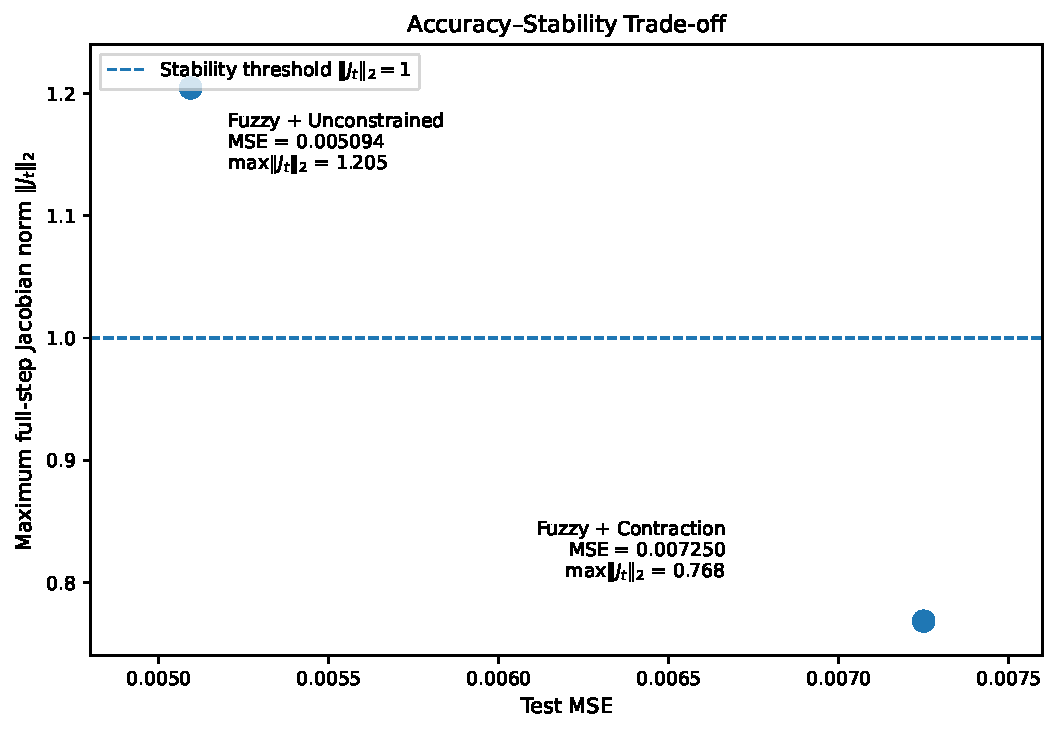
\includegraphics[width=0.85\linewidth]{Fig5_accuracy_stability.pdf}
		\caption{Accuracy--stability trade-off between the contractively constrained and unconstrained fuzzy models. The unconstrained model achieves lower test MSE but has a maximum full-step Jacobian norm above one, whereas the constrained model maintains a maximum norm below one.}
		\label{fig:accuracy_stability}
	\end{figure}
	
	The comparison demonstrates that the contraction constraint introduces an explicit accuracy--stability trade-off rather than directly improving forecasting accuracy. Removing the constraint gives the recurrent model greater predictive flexibility and lower error, but this comes at the cost of losing the contraction property. Conversely, the constrained model maintains the prescribed dynamical structure and provides the stability guarantee established in Section~\ref{sec:stability}.
	
	% ------------------------------------------------------------
	% 6.8 Full-Step Jacobian Verification
	% ------------------------------------------------------------
	
	\subsection{Full-Step Jacobian Verification}
	\label{subsec:jacobian_verification_results}
	
	The protocol-matched V4 experiment provides a direct empirical evaluation of the full-step recurrent Jacobian. For the contractively constrained fuzzy model, the mean Jacobian spectral norm is 0.653339, the 95th percentile is 0.725517, and the maximum observed value is 0.768368. No evaluated step exceeds one, and no theoretical-bound violations are observed. In contrast, the unconstrained fuzzy model has a mean Jacobian norm of 1.053622, a 95th percentile of 1.080260, and a maximum of 1.204569, with the Jacobian exceeding one throughout the evaluated trajectory.
	
	\begin{figure}[t]
		\centering
		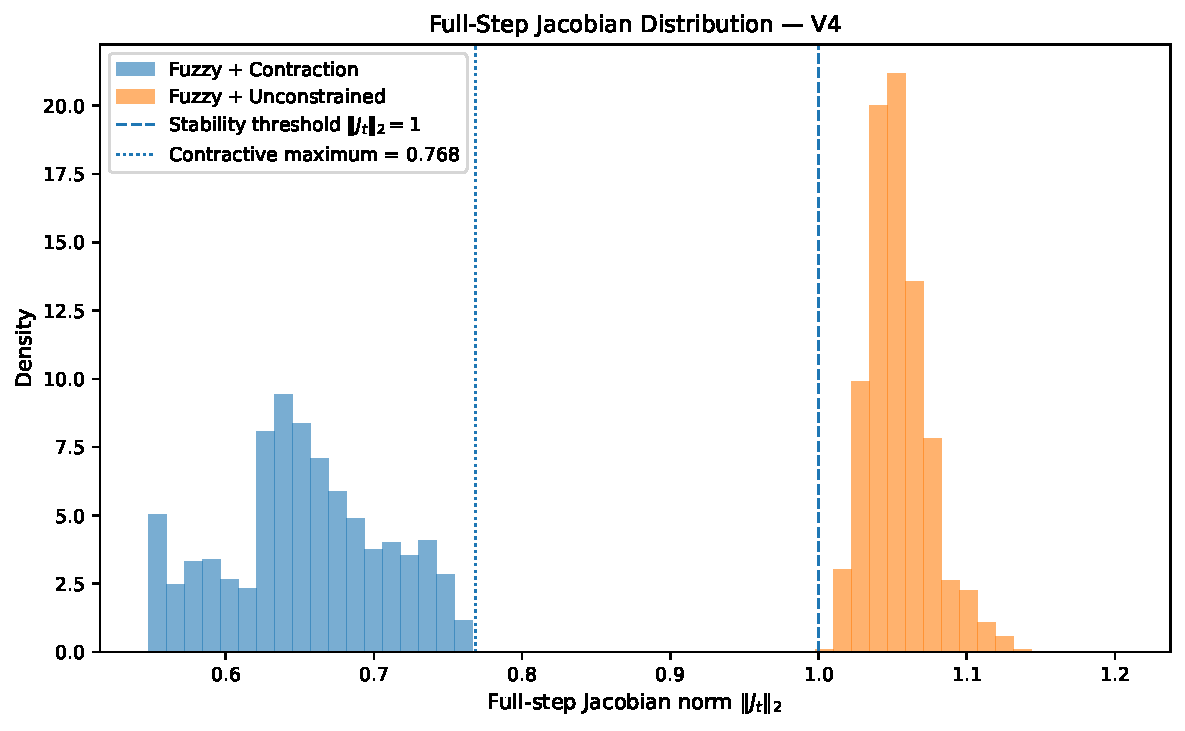
\includegraphics[
		width=0.95\linewidth
		]{paper_figures/Fig6_jacobian_distribution.pdf}
		\caption{Full-step Jacobian norm distributions from the protocol-matched V4 experiment. The contractively constrained model remains below the stability threshold $\lVert J_t\rVert_2=1$, whereas the unconstrained model is centered above the threshold.}
		\label{fig:jacobian_distribution}
	\end{figure}
	
	Across the three evaluated seeds, the contractively constrained model therefore exhibits zero observed Jacobian violations, whereas the unconstrained model records 30,000 violations over the evaluated steps. The recurrent spectral norm is also substantially different between the two configurations, with the constrained model remaining within the prescribed contractive region and the unconstrained model exceeding one. These observations provide empirical support for the theoretical contraction result, while the theoretical derivation itself remains independent of the particular evaluated trajectories.
	
	The analytical Jacobian calculation is additionally verified against automatic differentiation. The maximum absolute discrepancy between the analytical and automatic-differentiation Jacobians is $5.96\times10^{-8}$, indicating numerical agreement to near machine precision for the reported verification procedure. This cross-check supports the correctness of the Jacobian computation used to evaluate the empirical stability behavior.
	
	% ------------------------------------------------------------
	% 6.9 Contraction-parameter sensitivity
	% ------------------------------------------------------------
	
	\subsection{Contraction-Parameter Sensitivity}
	\label{subsec:kappa_sensitivity}
	
	The contraction parameter $\kappa$ controls the admissible spectral norm
	of the recurrent matrix and therefore the theoretical contraction margin.
	For fixed $\alpha_{\min}=0.02$, the bound derived in
	Section~\ref{sec:stability} is
	
	\begin{equation}
		q(\kappa)=1-\alpha_{\min}(1-\kappa).
	\end{equation}
	
	Thus, reducing $\kappa$ tightens the contraction guarantee, whereas
	increasing $\kappa$ weakens the contraction margin and moves the
	admissible recurrent dynamics closer to the unit-sensitivity boundary.
	Representative values are summarized in Table~\ref{tab:kappa_sensitivity}.
	
	\begin{table}[t]
		\centering
		\caption{Theoretical sensitivity of the contraction factor to $\kappa$
			for fixed $\alpha_{\min}=0.02$.}
		\label{tab:kappa_sensitivity}
		\begin{tabular}{ccc}
			\toprule
			$\kappa$ & $q=1-\alpha_{\min}(1-\kappa)$ & $1-q$ \\
			\midrule
			0.80 & 0.9960 & 0.0040 \\
			0.90 & 0.9980 & 0.0020 \\
			0.99 & 0.9998 & 0.0002 \\
			\bottomrule
		\end{tabular}
	\end{table}
	
	Figure~\ref{fig:kappa_sensitivity} visualizes the same relationship
	continuously. The stability guarantee remains valid for every
	$\kappa<1$, but the quantitative contraction margin becomes substantially
	smaller as $\kappa$ approaches one. In particular, changing $\kappa$
	from 0.90 to 0.99 reduces the theoretical margin $1-q$ by an order of
	magnitude, from 0.002 to 0.0002, whereas changing it to 0.80 doubles
	the margin to 0.004. These values characterize the theoretical
	stability consequence of $\kappa$ but do not by themselves establish a
	corresponding change in forecasting error.
	
	\begin{figure}[t]
		\centering
		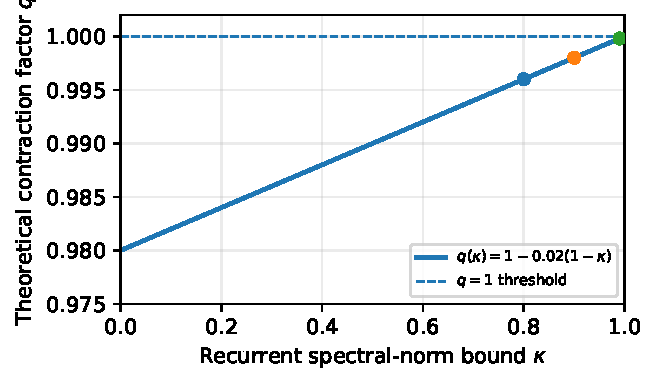
\includegraphics[width=0.95\linewidth]
		{Fig7_kappa_sensitivity.pdf}
		\caption{Theoretical contraction factor $q$ as a function of the
			recurrent spectral-norm bound $\kappa$ for fixed
			$\alpha_{\min}=0.02$. Lower $\kappa$ values provide a larger contraction
			margin, while $q$ approaches one as $\kappa$ approaches one.}
		\label{fig:kappa_sensitivity}
	\end{figure}
	
	The present analysis should therefore be interpreted as a theoretical
	sensitivity study rather than a full empirical hyperparameter sweep.
	A statistically powered multi-seed retraining study over multiple
	$\kappa$ values remains an important direction for future work.
	% ------------------------------------------------------------
	% Summary of Results
	% ------------------------------------------------------------
	
	\subsection{Summary of Experimental Findings}
	\label{subsec:results_summary}
	
	Taken together, the experiments support four main findings. First, adaptive temporal scaling provides the dominant forecasting improvement relative to a fixed update rate. Second, fuzzy interpolation provides a smaller additional improvement in the standard forecasting and regime-shift settings, although this advantage is not uniform under extreme data scarcity. Third, the contraction constraint reduces predictive flexibility and therefore introduces an accuracy--stability trade-off rather than an accuracy gain. Fourth, the protocol-matched V4 Jacobian analysis is consistent with the theoretical contraction guarantee, with the constrained model remaining strictly below the unit Jacobian threshold throughout the evaluated trajectories.
	
	% ============================================================
	% 7. Discussion
	% ============================================================
	
	\section{Discussion}
	\label{sec:discussion}
	
	\subsection{Predictive Contribution of Adaptive Temporal Scaling}
	\label{subsec:adaptive_contribution}
	
	The experimental results indicate that adaptive temporal scaling is the principal source of the predictive improvement achieved by FAC-RNN. In the main forecasting experiment, the mean test MSE decreases from 0.008253 for the fixed update-rate baseline to 0.007372 for the nonfuzzy adaptive model, demonstrating that allowing the recurrent update rate to vary with observable temporal context produces a substantial improvement in forecasting accuracy. The fuzzy adaptive configuration further reduces the MSE to 0.007250, but the additional gain over the nonfuzzy adaptive model is comparatively small. This pattern is also confirmed by the context ablation, where replacing the fixed update with a learned context-dependent coefficient produces the largest performance change.
	
	The results suggest that the temporal update rate $\alpha_t$ should be viewed as the primary adaptive mechanism of the architecture. Rather than forcing every observation to modify the hidden state by the same amount, FAC-RNN allows the recurrent dynamics to regulate the degree of state retention and responsiveness according to the observed context. Small values of $\alpha_t$ favor preservation of the previous hidden representation, whereas larger values increase the contribution of the newly computed nonlinear state. This mechanism provides a simple dynamical interpretation of the recurrent update and offers a direct connection between observable temporal behavior and hidden-state evolution.
	
	\subsection{Role of Fuzzy Interpolation}
	\label{subsec:fuzzy_role}
	
	Fuzzy interpolation provides a secondary but measurable contribution to predictive performance, although its benefit depends on the available amount of training data. In the context ablation, the nonfuzzy value-plus-$\Delta$ configuration obtains a mean test MSE of 0.007679, while the fuzzy value-plus-$\Delta$ configuration reduces the MSE to 0.007518, corresponding to a 2.10\% improvement. The main forecasting comparison shows a similar pattern, with the fuzzy adaptive model improving the mean MSE by 1.66\% relative to the nonfuzzy adaptive model. These results indicate that fuzzy interpolation contributes useful additional flexibility while preserving a bounded and smooth mapping from temporal context to the update rate.
	
	The policy surface in Fig.~\ref{fig:fuzzy_policy} provides a complementary view of this mechanism. The learned mapping from $(y_t,\Delta_t)$ to $\alpha_t$ varies continuously across the evaluated context space, reflecting the interpolation of neighboring fuzzy rules rather than a hard rule-selection mechanism. This smoothness is desirable for a recurrent dynamical system because small changes in observable context do not induce discontinuous changes in the temporal update. Nevertheless, the present experiments do not establish a unique semantic interpretation of the individual fuzzy rules, and the contribution of fuzzy interpolation should therefore be interpreted primarily as a smooth policy parameterization.
	
	\subsection{Adaptive Behavior Across Dynamical Regimes}
	\label{subsec:regime_behavior}
	
	The regime analysis provides evidence that the learned temporal update rate is context dependent rather than globally fixed. The mean values of $\alpha_t$ are approximately 0.391, 0.424, and 0.389 for the three regimes, respectively, with the second regime exhibiting the highest average update rate. This variation is consistent with the intended role of temporal scaling, namely, to permit different degrees of responsiveness under different local dynamical conditions. The regime-shift forecasting experiment further shows that both adaptive models outperform the fixed-rate baseline, with the fuzzy model providing an additional 1.57\% reduction in test MSE relative to the nonfuzzy adaptive model.
	
	These findings support the use of adaptive temporal modulation across changing dynamical conditions, but they should not be interpreted as evidence that FAC-RNN explicitly detects regime boundaries or reacts faster to regime transitions than alternative adaptive controllers. The available transition analysis does not provide sufficiently strong evidence for a systematic reduction in adaptation lag. The more defensible conclusion is that the proposed controller learns different temporal response characteristics for different dynamical regimes.
	
	\subsection{Accuracy--Stability Trade-off}
	\label{subsec:tradeoff_discussion}
	
	The stability ablation reveals a clear trade-off between predictive flexibility and dynamical control. The unconstrained fuzzy model achieves a lower mean test MSE of 0.005094, compared with 0.007250 for the contractively constrained model. However, this improved predictive performance is accompanied by a recurrent spectral norm exceeding one and full-step Jacobian norms that cross the unit threshold. The constrained model therefore sacrifices some forecasting accuracy in exchange for an explicit restriction on recurrent sensitivity.
	
	This trade-off is an expected consequence of imposing a contraction constraint rather than a failure of the proposed method. The purpose of the constraint is not to minimize the forecasting loss directly, but to restrict the recurrent transition to a region for which a uniform contraction guarantee can be established. The results therefore demonstrate that predictive accuracy and dynamical stability represent distinct objectives. A model may obtain lower error by exploiting more flexible recurrent dynamics while simultaneously losing the formal stability property targeted by FAC-RNN.
	
	\subsection{Theoretical Guarantee and Empirical Verification}
	\label{subsec:theory_empirical}
	
The theoretical analysis establishes a one-step Jacobian bound of the form $\lVert J_t\rVert_2\leq1-\alpha_{\min}(1-\kappa)$. With $\alpha_{\min}=0.02$ and $\kappa=0.9$, this gives the uniform contraction factor $q=0.998<1$. The significance of this result is that the bound is derived directly from the architecture and parameter constraints and does not depend on the particular trajectory used during evaluation. It therefore establishes a formal dynamical property of the admissible recurrent state transition.

	The protocol-matched V4 experiment provides an empirical verification of this theoretical condition. The contractively constrained model has a mean full-step Jacobian norm of 0.653339, a 95th percentile of 0.725517, and a maximum of 0.768368, with zero observed steps exceeding one and zero observed theoretical-bound violations. In contrast, the unconstrained model has a mean Jacobian norm of 1.053622, a 95th percentile of 1.080260, and a maximum of 1.204569, with all 30,000 evaluated steps exceeding the unit threshold. The agreement between the analytical and automatic-differentiation Jacobians, with a maximum discrepancy of $5.96\times10^{-8}$, further supports the numerical reliability of the empirical stability analysis.
	
	It is important to distinguish the theoretical and empirical roles of these results. The contraction theorem provides the formal guarantee under the specified assumptions, while the V4 experiment demonstrates that the trained model and evaluated trajectories exhibit the predicted behavior in practice. The empirical observation that all measured Jacobian norms remain below one for the constrained model is therefore supporting evidence for the theoretical analysis rather than a substitute for the proof.
	
\subsection{Statistical Robustness of the Main Comparison}
\label{subsec:statistical_robustness}

The three-seed main comparison exhibits relatively small dispersion for all three controlled models, with test-MSE standard deviations of 0.000237, 0.000198, and 0.000018 for the fixed, nonfuzzy, and fuzzy configurations, respectively. The paired test between FAC-RNN and the fixed baseline yields $p=0.0207$, while the corresponding comparison with the nonfuzzy adaptive model yields $p=0.4289$; the Wilcoxon test for the latter comparison gives $p=0.50$. Thus, the evidence for adaptive temporal scaling over the fixed update rate is stronger than the evidence for a statistically significant advantage of fuzzy interpolation over the matched nonfuzzy controller. Because the inference is based on only three seeds, these tests are treated as exploratory and are reported together with effect sizes and dispersion rather than as definitive population-level significance claims.

\subsection{Behavior Under Data Scarcity}
\label{subsec:data_scarcity_discussion}

The data-scarcity experiments reveal a particularly strong benefit from adaptive temporal scaling when the number of training windows is reduced. The nonfuzzy adaptive model substantially outperforms the fixed baseline at all evaluated training sizes, whereas the fuzzy model does not consistently provide the best result at the smallest sample sizes. For example, at 1,000 training windows, the nonfuzzy model achieves an MSE of 0.018869 compared with 0.043039 for the fuzzy model, while at 9,000 windows the fuzzy configuration achieves the lowest MSE of 0.007599.

To further characterize this behavior, we compared the theoretical context-sensitivity bounds of the fuzzy and nonfuzzy temporal policies. For the fuzzy controller, $L_F\leq\frac{\alpha_{\max}-\alpha_{\min}}{2\sigma^2}\|W_2\|_2\|W_1\|_2$, whereas the corresponding nonfuzzy controller satisfies $L_{NF}\leq\frac{\alpha_{\max}-\alpha_{\min}}{4}\|W_2\|_2\|W_1\|_2$. Across the four training-set sizes, the estimated fuzzy-policy sensitivity bound is substantially larger than the corresponding nonfuzzy bound. The ratio $L_F/L_{NF}$ ranges from 3.87 to 4.23, indicating that the fuzzy controller has approximately four times greater potential sensitivity to changes in the observable temporal context.

This structural difference is consistent with the observed scarcity behavior. Under the most severe scarcity condition of 1,000 training windows, the fuzzy controller exhibits a substantially larger prediction error than the nonfuzzy adaptive controller. As the training set increases, this disadvantage progressively decreases, and at 9,000 windows the fuzzy controller slightly outperforms the nonfuzzy alternative. These observations suggest that the additional context-sensitive flexibility introduced by fuzzy interpolation may require sufficient data to be exploited reliably, whereas the nonfuzzy adaptive mapping is more robust under extreme data scarcity.

Importantly, the sensitivity analysis does not establish a monotonic relationship between training-set size and $L_F$. The fuzzy sensitivity bound is highest at 1,000 windows but remains of similar magnitude at the larger training sizes. Therefore, the bound should not be interpreted as a complete causal explanation of the data-scarcity trend. Rather, it provides a structural characterization of the greater context sensitivity of the fuzzy temporal policy and identifies a plausible mechanism through which additional adaptive flexibility can interact with finite-sample effects. The empirical results indicate that this flexibility is disadvantageous under extreme scarcity but becomes beneficial when sufficient training information is available.

	\subsection{Implications for Recurrent Dynamical Modeling}
	\label{subsec:implications}
	
	The results suggest that adaptive temporal scaling and contraction should be regarded as complementary design objectives rather than interchangeable alternatives. The adaptive coefficient controls how quickly the hidden representation responds to new observations, while the recurrent contraction constraint limits the sensitivity of the underlying nonlinear transition. This separation makes it possible to study predictive adaptation and dynamical stability independently and to quantify the trade-off between them.
	
	More broadly, FAC-RNN demonstrates a design pattern in which an interpretable temporal control variable is embedded directly into the recurrent state equation and coupled with an explicit operator-level stability condition. The resulting architecture does not rely solely on empirical observation to characterize its recurrent behavior; instead, a formal bound is available from the model construction itself. At the same time, the experiments show that imposing such a bound can restrict predictive flexibility, emphasizing that dynamical certification and forecasting accuracy should be evaluated as distinct objectives.
	
\subsection{External Generalization and Modern Baselines}
\label{subsec:external_generalization_discussion}

The real-world benchmark provides an important qualification to the controlled nonlinear results. On the El Nino monthly sea-surface-temperature series, FAC-RNN does not achieve the lowest forecasting error; the fixed update-rate baseline performs best, while the Transformer is the strongest modern baseline in this experiment. This outcome indicates that the adaptive and contractive design should not be interpreted as universally improving predictive accuracy across datasets. Instead, the principal empirical contribution of the architecture is the demonstrated separation between adaptive temporal modulation and explicit recurrent contraction, together with a measurable accuracy--stability trade-off. The real-world experiment therefore strengthens the paper by testing the architecture outside the synthetic setting while also making the limits of its predictive generalization explicit.

	\subsection{Limitations}
	\label{subsec:limitations}
	
	Several limitations should be acknowledged. First, although the study now includes an external real-world benchmark, the real-world evaluation is based on a single univariate El Nino dataset and therefore does not establish broad cross-domain generalization. Second, the experiments focus primarily on one-step-ahead forecasting and do not establish that the proposed architecture solves general long-term memory problems. Third, fuzzy interpolation is not uniformly superior under extreme data scarcity, which limits the scope of claims regarding its robustness in low-data settings. Fourth, the main statistical comparisons rely on only three training seeds, so inferential results should be interpreted as exploratory. Fifth, the present analysis establishes contraction of the hidden-state transition under the stated assumptions, but this should not be interpreted as a direct guarantee of forecasting accuracy, task-level stability, or absence of all gradient-related phenomena in a complete training system.
	
	Taken together, the findings support FAC-RNN as a recurrent forecasting framework that explicitly separates three roles: adaptive temporal scaling for predictive responsiveness, fuzzy interpolation for smooth context-dependent control, and contraction constraints for dynamical certification. The main controlled experiments show that adaptive temporal scaling is the dominant source of predictive improvement, while fuzzy interpolation provides a smaller gain whose statistical significance is not established with three seeds and whose benefit depends on data availability. The sensitivity analysis further shows that the fuzzy temporal policy has a substantially larger potential sensitivity to observable context than the nonfuzzy alternative, helping to characterize why its additional flexibility is not uniformly beneficial under extreme data scarcity. The external El Nino benchmark demonstrates that these controlled gains do not automatically translate into superior real-world forecasting accuracy, reinforcing the importance of evaluating predictive performance and dynamical certification as distinct objectives. Meanwhile, the contraction constraint introduces a measurable accuracy--stability trade-off. The theoretical contraction bound and the protocol-matched Jacobian measurements jointly provide evidence that the proposed recurrent dynamics can be both adaptive and explicitly constrained, while the external benchmark clarifies the current limits of predictive generalization.



	% ============================================================
	% 8. Conclusion
	% ============================================================
	
	\section{Conclusion}
	\label{sec:conclusion}
	
	This paper introduced FAC-RNN, a recurrent neural network architecture that combines adaptive temporal scaling, fuzzy context-dependent interpolation, and an explicit contraction constraint within a unified dynamical framework for time-series forecasting. The proposed recurrent update uses a context-dependent coefficient $\alpha_t$ to regulate the balance between state retention and response to newly computed information, while fuzzy interpolation provides a smooth bounded mapping from observable temporal context to the adaptive update rate.
	
	The experimental results show that adaptive temporal scaling is the main source of the predictive improvement in the controlled nonlinear benchmark. In the main forecasting experiment, FAC-RNN achieves a mean test MSE of 0.007250 $\pm$ 0.000018, corresponding to a 12.16\% reduction relative to the fixed update-rate baseline and a 1.66\% lower mean MSE relative to the nonfuzzy adaptive model; however, the latter difference is not statistically significant with three seeds ($p=0.4289$). The context ablation further confirms that the largest improvement arises from replacing the fixed update mechanism with an adaptive one, while fuzzy interpolation provides a smaller additional gain. The regime analysis also demonstrates that the learned update rate varies across different nonlinear dynamical regimes, supporting the use of context-dependent temporal modulation.
	
	In addition to predictive adaptation, FAC-RNN explicitly constrains the recurrent dynamics through $\lVert W_h\rVert_2\leq\kappa<1$ and $\alpha_t\geq\alpha_{\min}>0$. These conditions yield the theoretical contraction bound
	\begin{equation}
		\lVert J_t\rVert_2
		\leq
		1-\alpha_{\min}(1-\kappa)
		=
		0.998
		<1,
	\end{equation}
	for the experimental values $\kappa=0.9$ and $\alpha_{\min}=0.02$. The protocol-matched full-step Jacobian experiment provides consistent empirical evidence, with a maximum observed Jacobian norm of 0.768 for the contractively constrained model and zero observed violations of the unit threshold, compared with a maximum of 1.205 and 100\% threshold violations for the unconstrained counterpart.
	
	The results therefore establish an explicit accuracy--stability trade-off rather than suggesting that contraction directly improves forecasting error. The unconstrained model achieves greater predictive flexibility and lower MSE, whereas the constrained FAC-RNN provides a formal and empirically supported contraction property. This distinction highlights the main value of FAC-RNN as a stability-aware recurrent design in which adaptive temporal responsiveness and dynamical certification are treated as complementary objectives.
	
	The external real-world benchmark shows that FAC-RNN does not uniformly outperform simpler or attention-based forecasting baselines, so the current evidence supports a stability-aware architectural contribution rather than universal predictive superiority. The study remains limited by one real-world univariate dataset, primarily one-step-ahead forecasting, and a small number of training seeds for the main statistical comparison. Future work will extend the evaluation to additional real-world domains, longer forecasting horizons, broader modern forecasting architectures, and systematic hyperparameter and contraction-sensitivity studies to assess the generality and practical utility of the proposed design.
	
	% ============================================================
	% References
	% ============================================================
	

\bibliographystyle{IEEEtran}
\bibliography{ref}
	
\end{document}